\section{Short bodies}
\label{sec:short}

XX per AR=2 FISSA RE FLUSSO BASE E ALZA RE STABILIT PER VEDERE SE QUI SI STABILIZZA O MENO XX

We begin by examining short bodies with aspect ratios in the range $1 \le \AR <3$, to assess how a modest increase in $\AR$ alters the bifurcation structure and the sequence in which flow modes become unstable, relative to the well-studied $\AR=1$ case. This analysis complements the work of \cite{choi-yang-2014}, who investigated the onset of secondary instabilities for bodies ranging from a flat plate normal to the flow ($\AR \rightarrow 0$) to a square cylinder ($\AR=1$).

\subsection{The base flow}

\begin{figure}
  \centering
  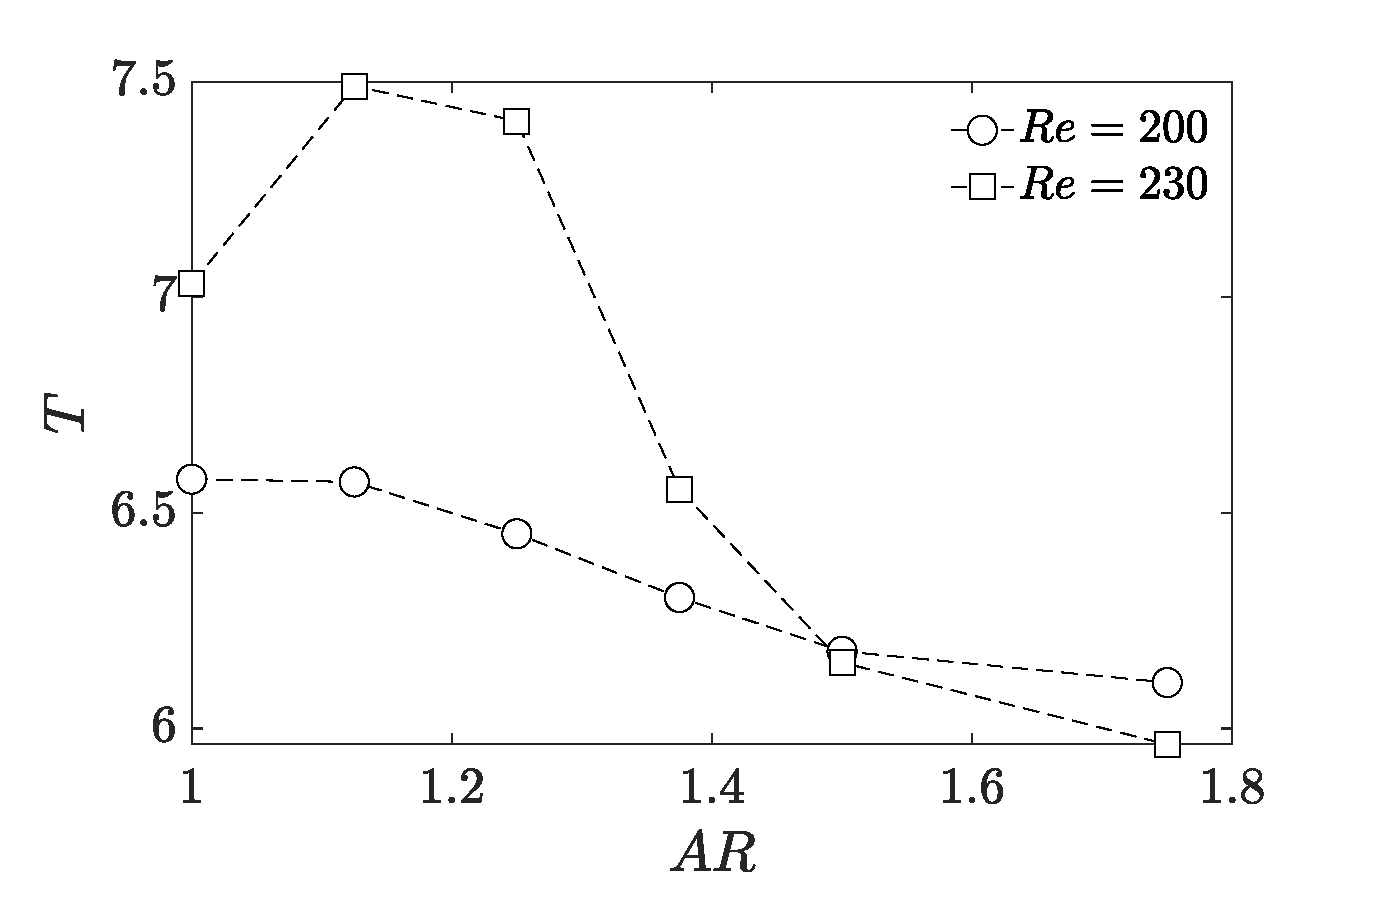
\includegraphics[width=0.49\textwidth]{./fig/AR1s/T_AR.eps}
  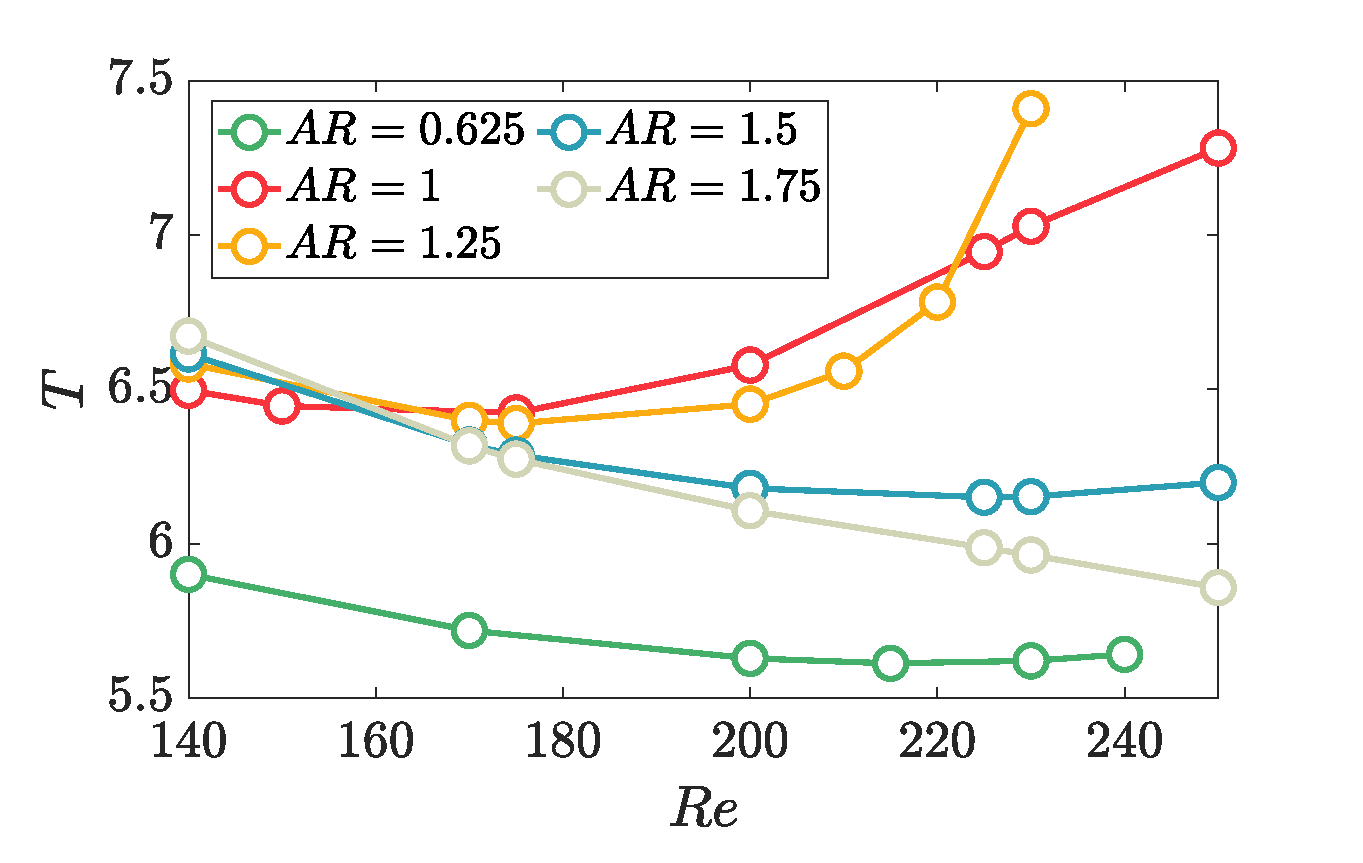
\includegraphics[width=0.49\textwidth]{./fig/AR1s/T_Re.eps}
  \caption{Base-flow period as a function of $\AR$ and $Re$. Left: dependence of $T$ on $Re$ for $1 \le \AR \le 1.75$. Right: dependence of $T$ on $\AR$ for $Re=200$ and $Re=230$. XX MODIFICARE FIGURA USANDO PALLINI PIENI QUANDO RIATTACCA IN MEDIA E VUOTI QUANDO NON RIATTACCA IN MEDIA; AGGIUNGERE CON UN INSET DIPENDENZA DELLA BOLLA DI RICIRCOLO MEDIA CON RE PER ALCUNI CASI PARTICOLARI. XX}
  \label{fig:T_Re_small}
\end{figure}
%

We begin by characterising the influence of aspect ratio $\AR$ and Reynolds number $Re$ on the periodic base flow. Figure \ref{fig:T_Re_small} shows the variation of the base-flow shedding period $T$ with both parameters. In figure \ref{fig:T_Re_small}(b), for $\AR=1.25$, results are not reported beyond $Re=240$, as the two-dimensional base flow loses periodicity near $Re \approx 250$ due to a Neimark–Sacker bifurcation (not shown for brevity).
%
The shedding period exhibits a strong dependence on both $\AR$ and $Re$. For the shortest bodies ($\AR \lessapprox 1$), the period $T$ varies only mildly with $Re$: for example, when $Re$ increases from $140$ to $230$, $T$ increases by approximately $2.2\%$ for $\AR=0.75$, see figure \ref{fig:T_Re_small}(b). In contrast, for intermediate ($1 \lessapprox \AR \lessapprox 1.5$) and longer bodies ($\AR \gtrapprox 1.5$), the variation is more pronounced. Over the same $Re$ range, $T$ increases by $12.6\%$ for $\AR=1.25$, while it decreases by $12.9\%$ for $\AR=3$.
%
When holding $Re$ fixed and varying $\AR$, figure~\ref{fig:T_Re_small}(a) shows that $T$ increases monotonically with $\AR$ for $Re \le 140$. At higher Reynolds numbers, however, $T$ displays a non-monotonic dependence on $\AR$, with a maximum around the intermediate $\AR \approx 1.25$. Interestingly, the dependence of $T$ on both $\AR$ and $Re$ mirrors that of the time-averaged wake recirculation length $\ell_w$ (see the inset in figure \ref{fig:T_Re_small}(v)), measured using the mean streamline defined by $\aver{\Psi_b} = 0$, where the streamfunction $\Psi_b$ satisfies $\bm{\nabla}^2 \Psi_b = - \omega$.

\begin{figure}
  \centering
  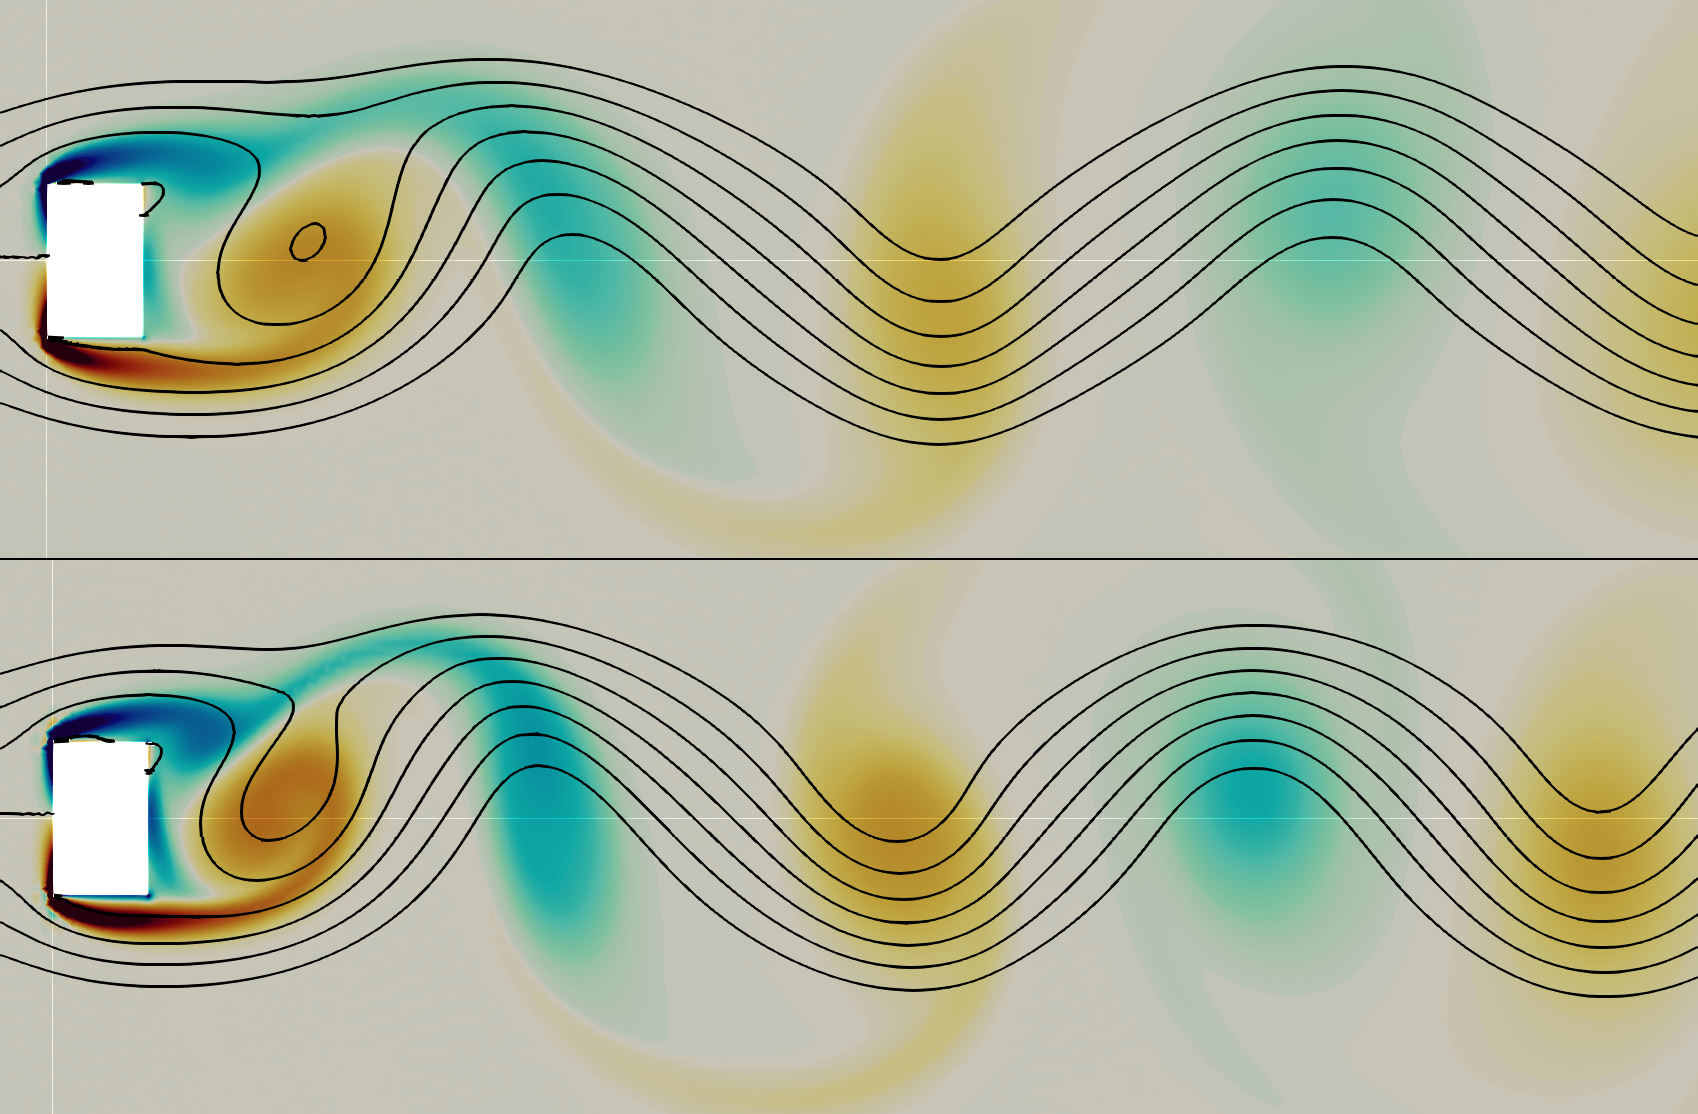
\includegraphics[width=0.49\textwidth]{./fig/AR1s/AR0p625_Re140_Re230_omegaz.png}
  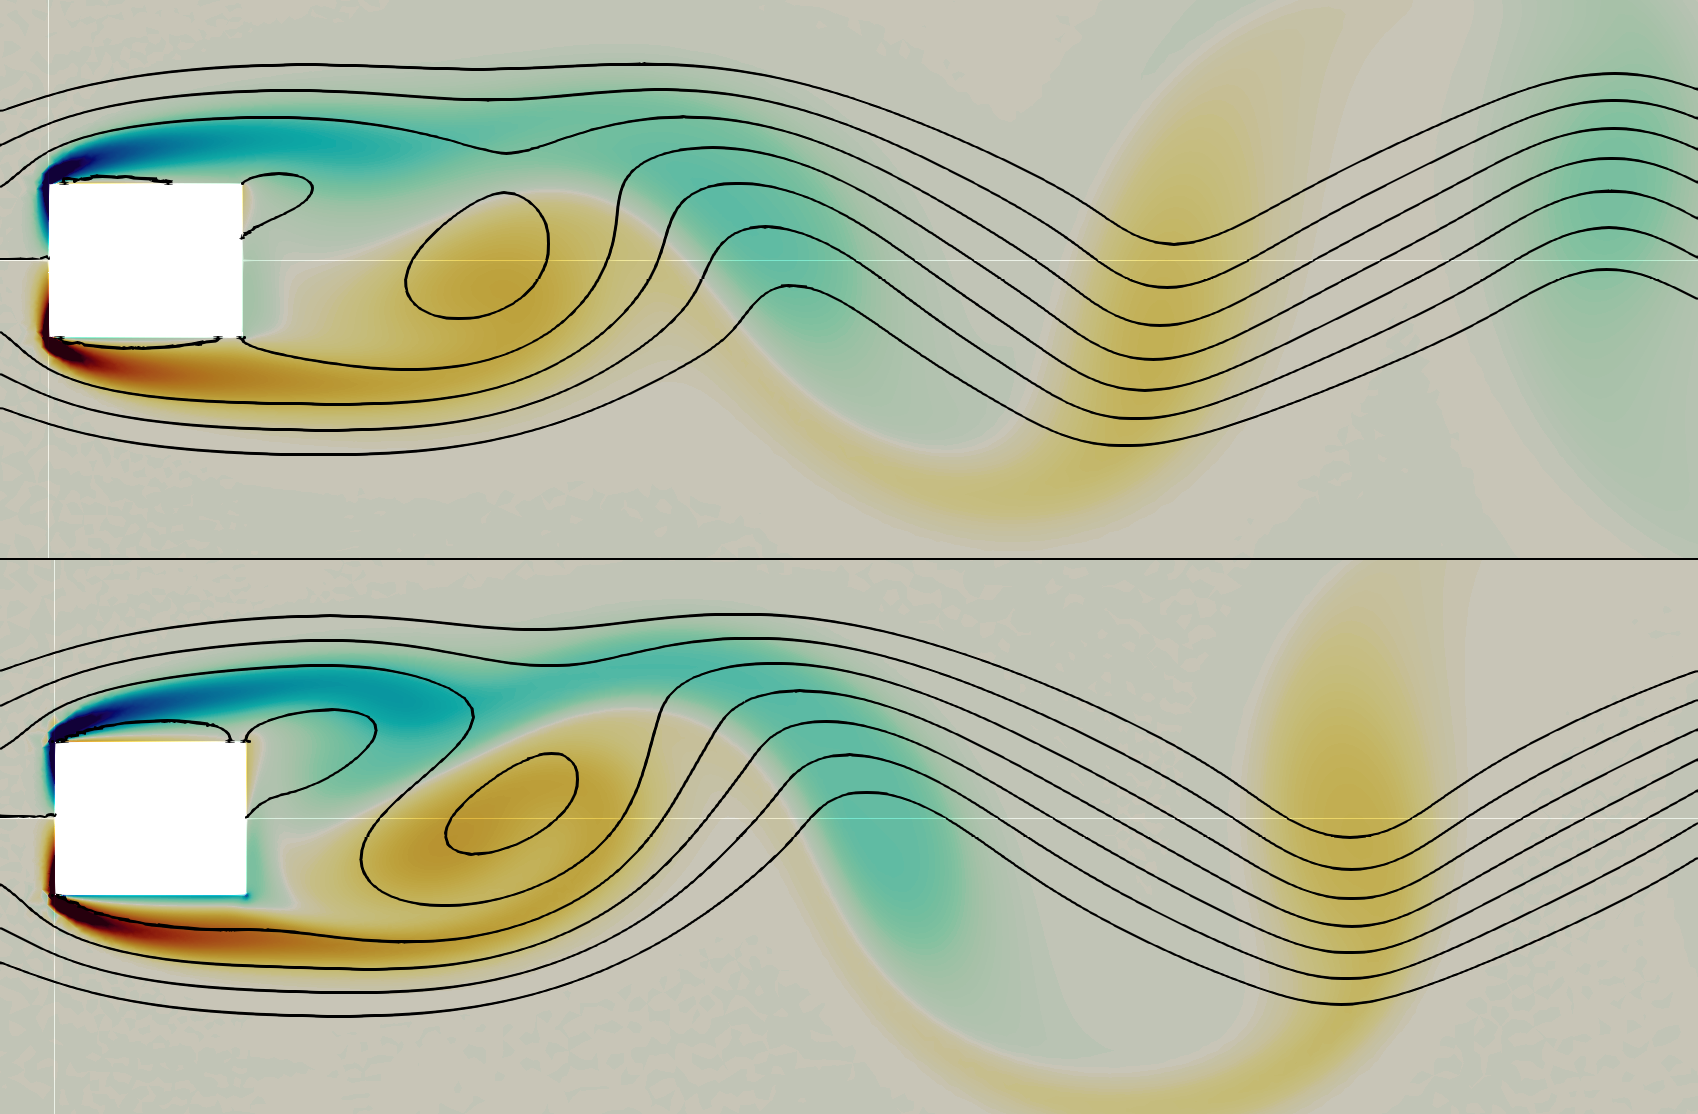
\includegraphics[width=0.49\textwidth]{./fig/AR1s/AR1p25_Re140_Re230_omegaz.png}
  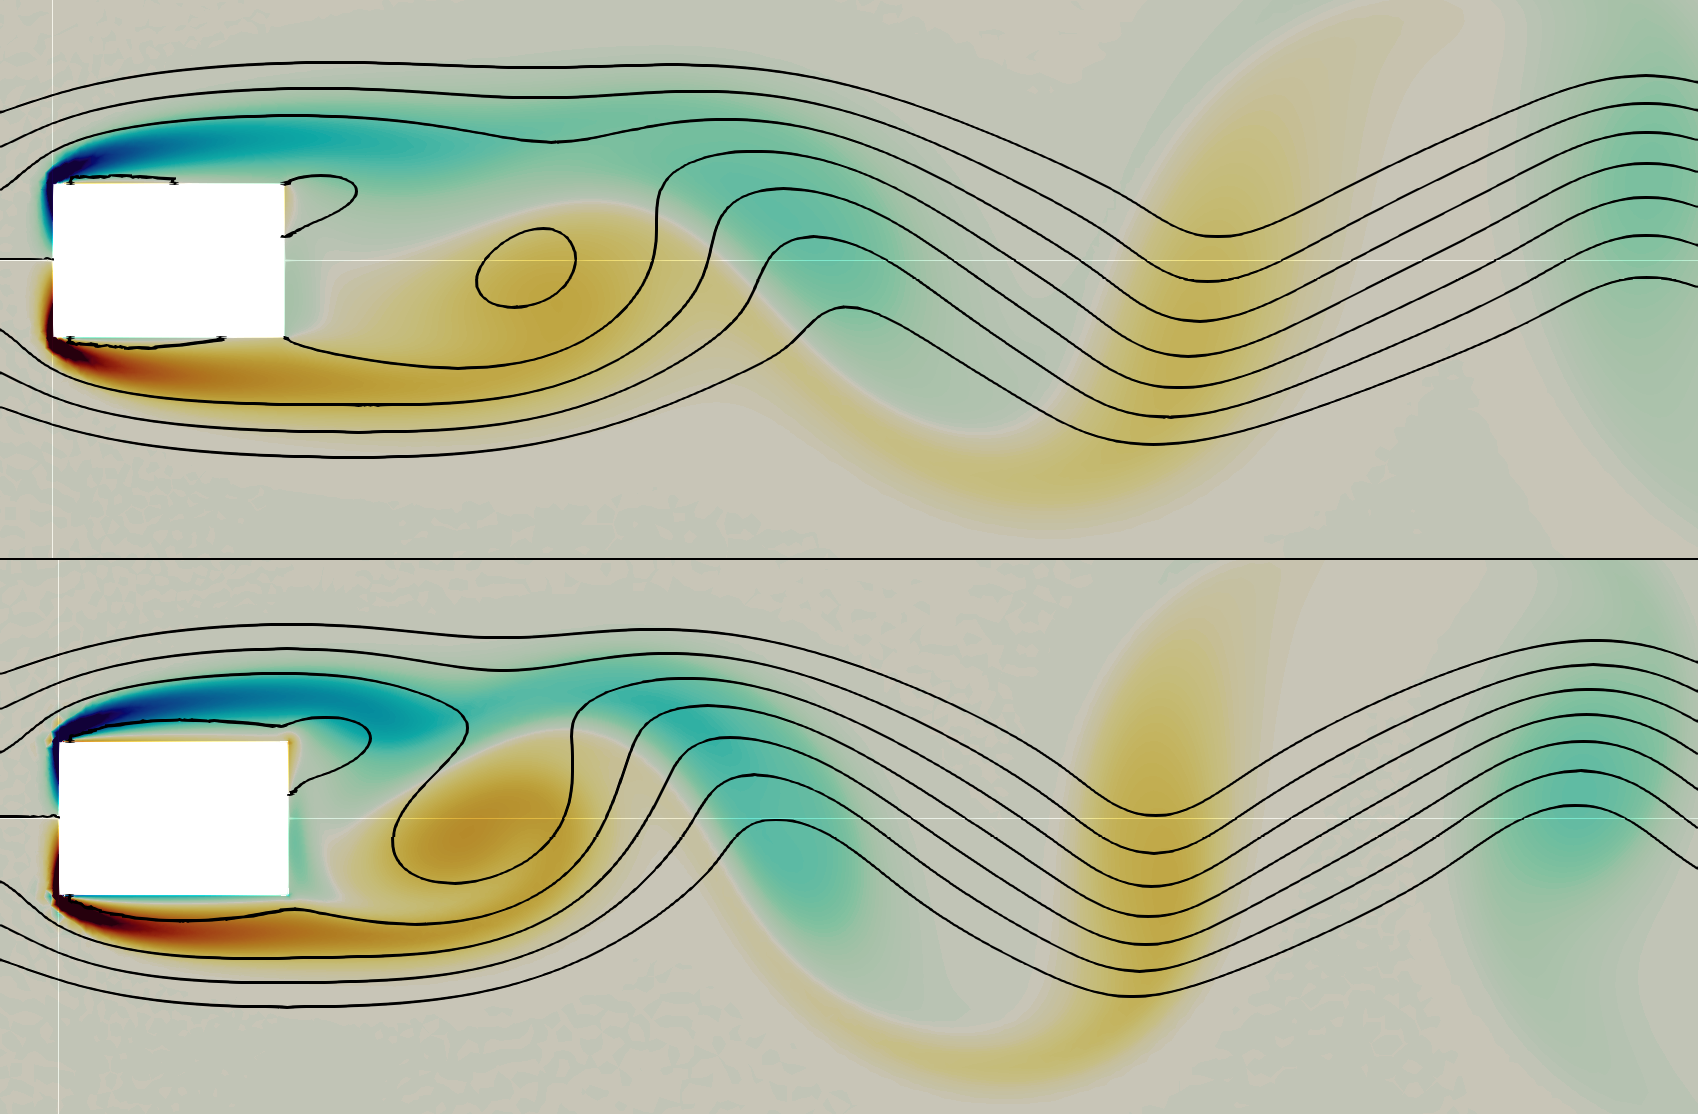
\includegraphics[width=0.49\textwidth]{./fig/AR1s/AR1p5_Re140_Re230_omegaz.png}
  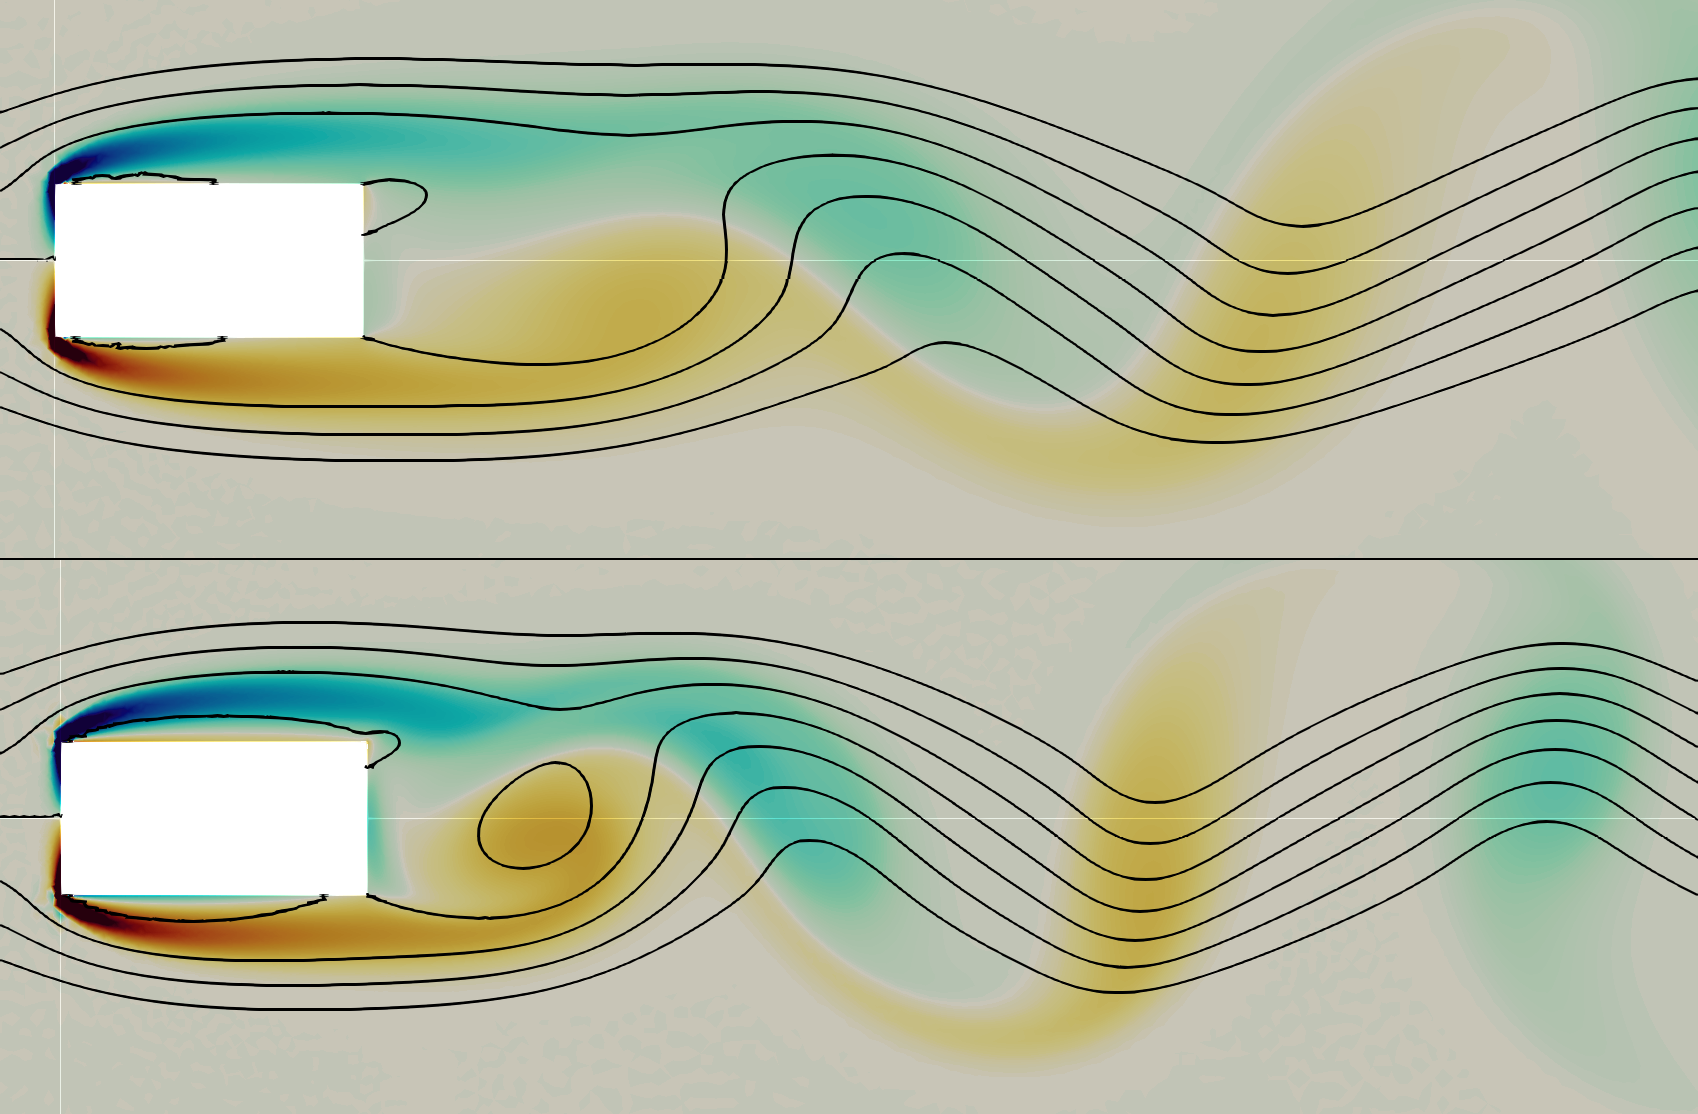
\includegraphics[width=0.49\textwidth]{./fig/AR1s/AR2_Re140_Re230_omegaz.png}
  \caption{Instantaneous visualisation of the flow for $Re=140$ (top) and $Re=230$ (bottom). Top left: $\AR=0.625$. Top right: $\AR=1.125$. Bottom left: $\AR=1.5$. Bottom right: $\AR=2$. The colour map denotes the spanwise vorticity in the $-10 \le \omega_z \le 10$ range. The black lines indicate the flow streamlines determined as isolines of $\psi$ spaces with $\pm 0.2$. XX IL CAMBIO DI ANDAMENTO DI $T$ SI VEDE QUANDO LA CORRENTE NON RIATTACCA PIU IN QUEL CASO COMINCIA DI NUOVO A CRESERE T. E' POSSIBILE VEDERLO, P.E. GUARDANDO IL CAMPO MEDIO XX}
  \label{fig:snap_Re140_Re230}
\end{figure}    


\begin{figure}
  \centering
  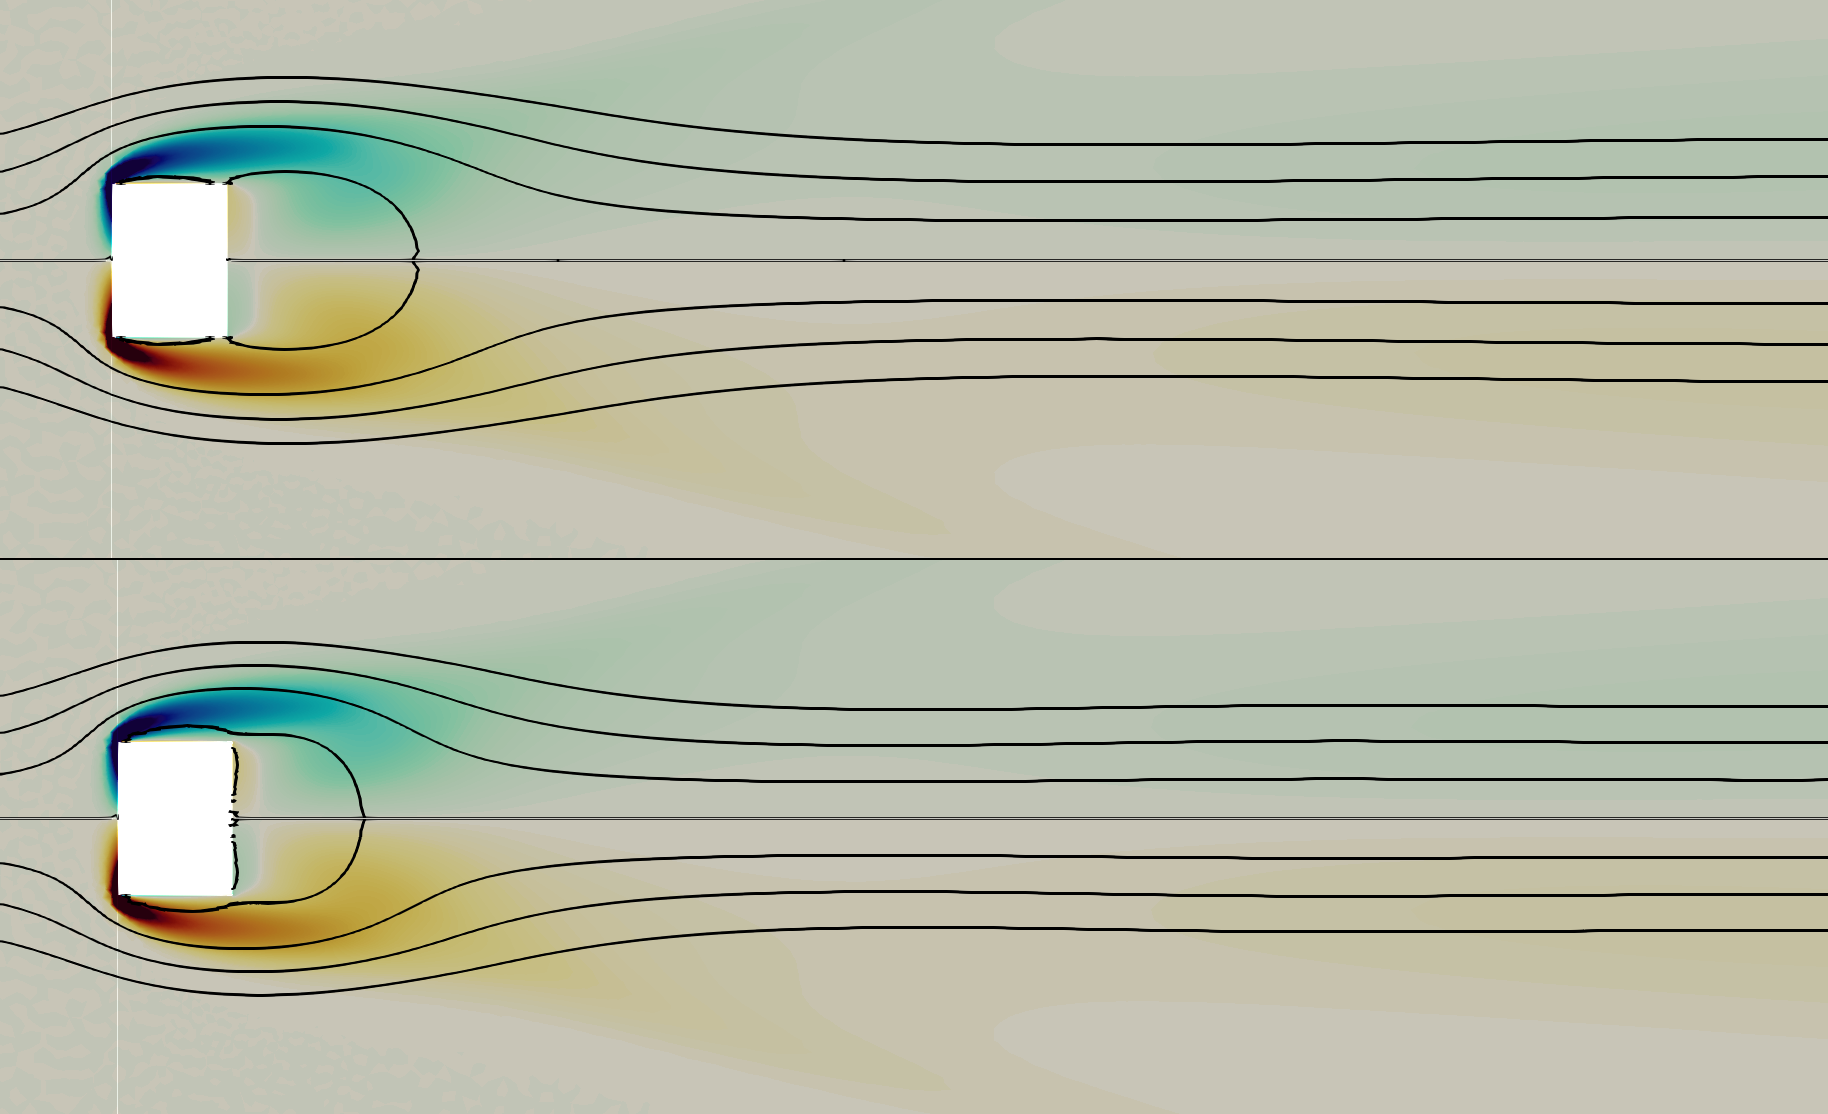
\includegraphics[width=0.49\textwidth]{./fig/AR1s/AR0p75_Re140_Re230_omegaz_Av.png}
  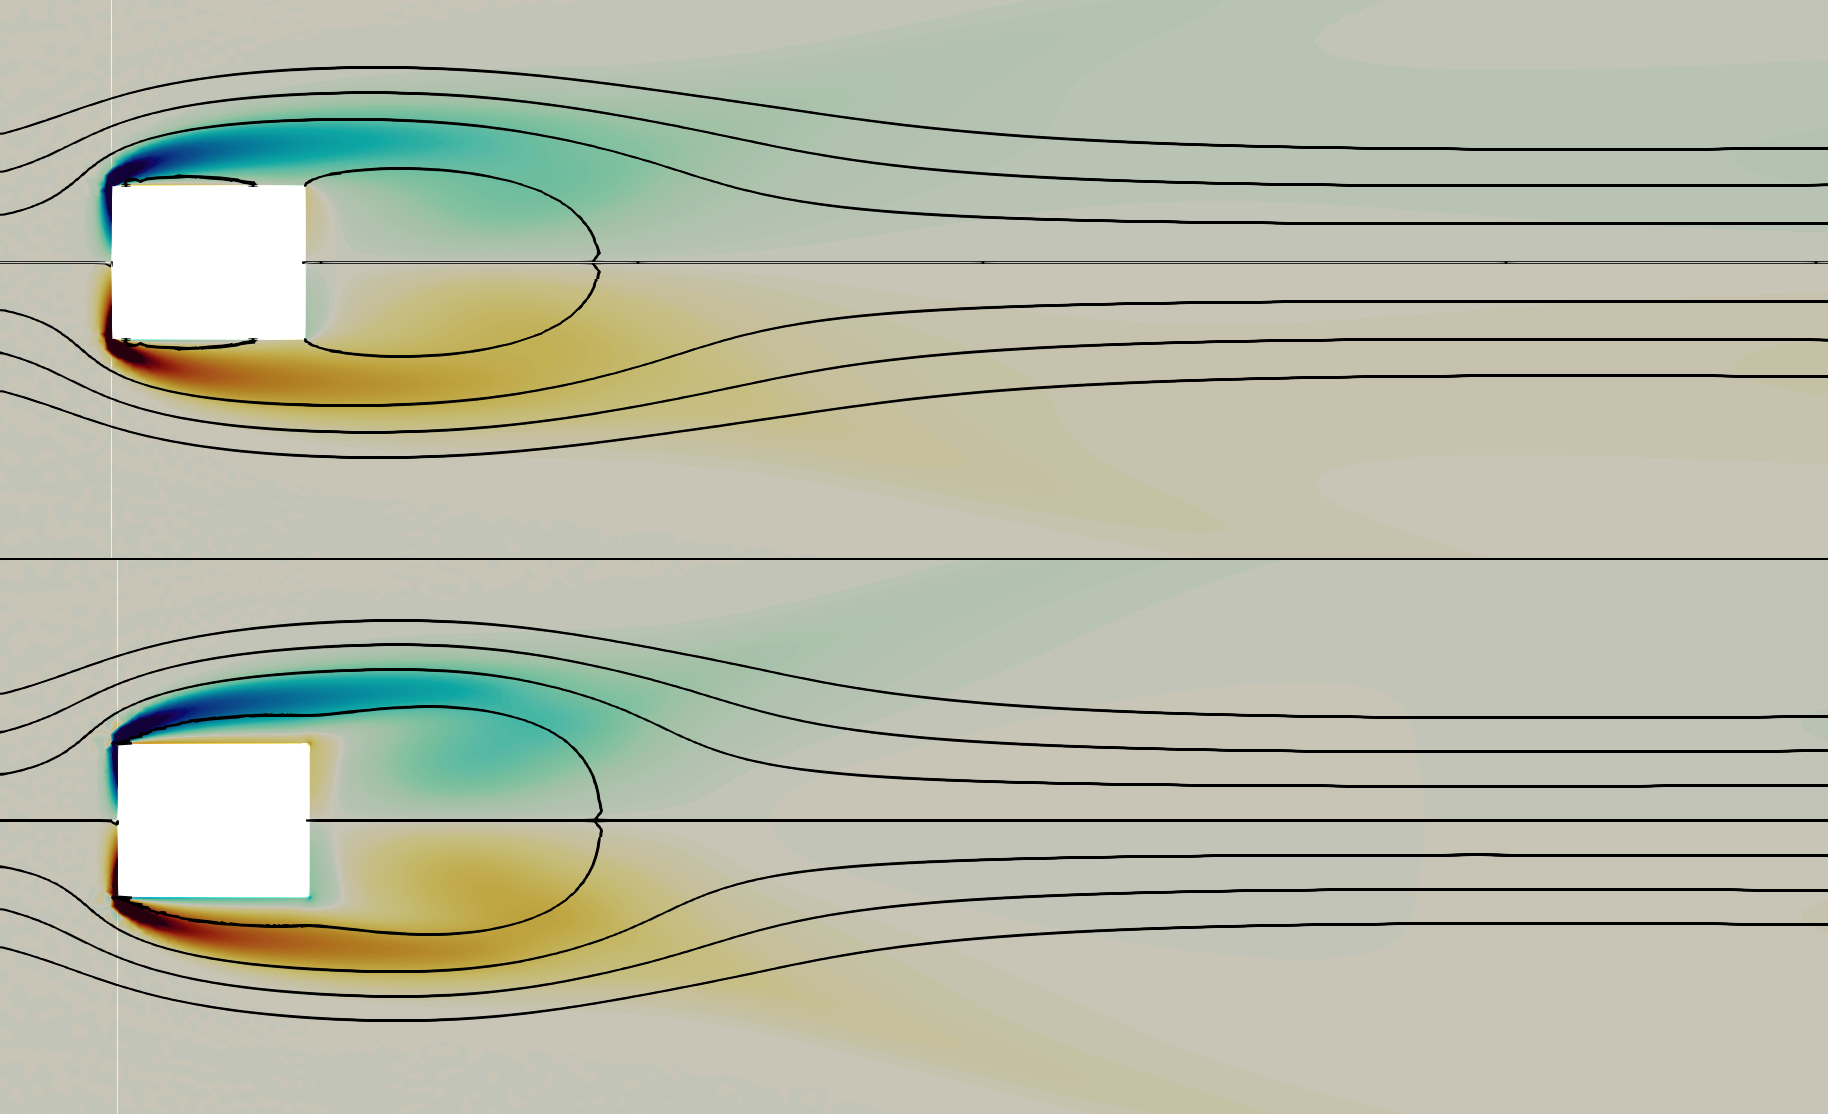
\includegraphics[width=0.49\textwidth]{./fig/AR1s/AR1p25_Re140_Re230_omegaz_Av.png}
  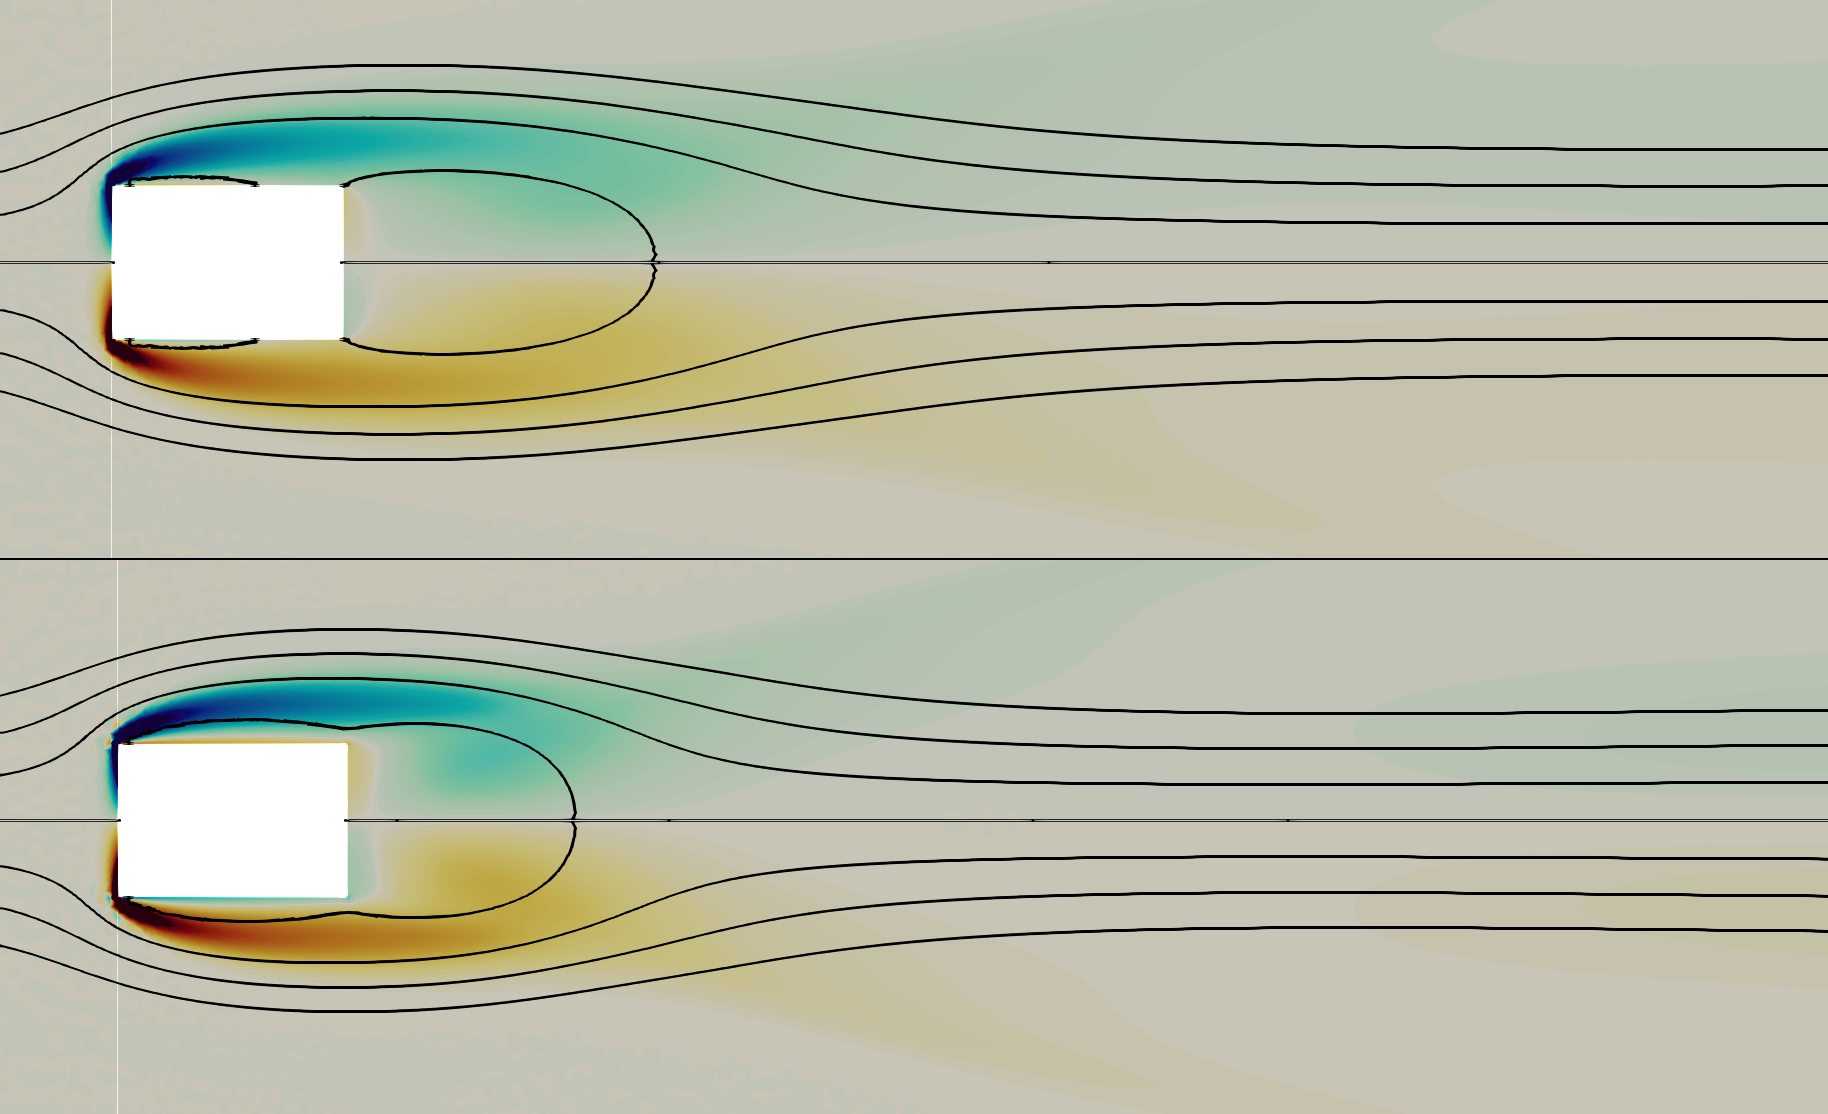
\includegraphics[width=0.49\textwidth]{./fig/AR1s/AR1p5_Re140_Re230_omegaz_Av.png}
  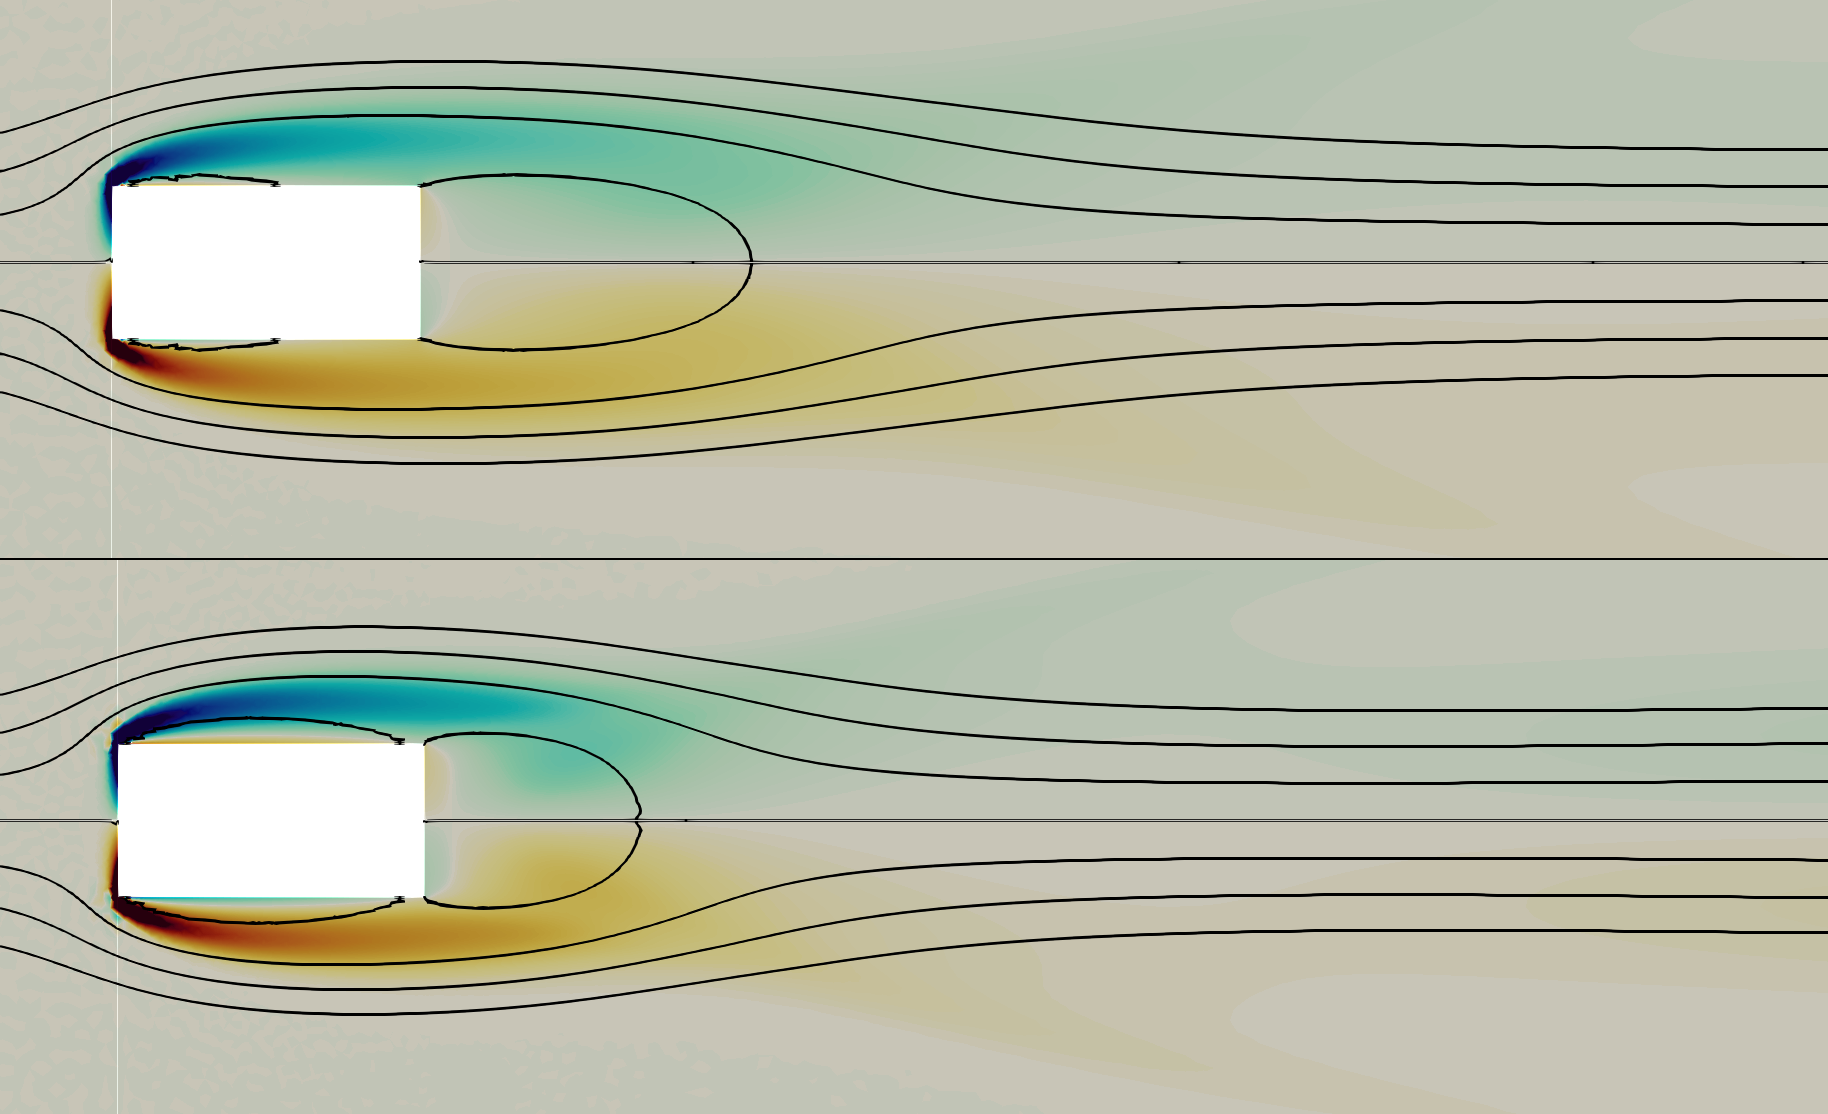
\includegraphics[width=0.49\textwidth]{./fig/AR1s/AR2_Re140_Re230_omegaz_Av.png}
  \caption{Visualisation of the mean flow for $Re=140$ (top) and $Re=230$ (bottom). Top left: $\AR=0.625$. Top right: $\AR=1.125$. Bottom left: $\AR=1.5$. Bottom right: $\AR=2$. The colour map denotes the spanwise vorticity in the $-10 \le \omega_z \le 10$ range. The black lines indicate the flow streamlines determined as isolines of $\psi$ spaces with $\pm 0.2$. XX IL CAMBIO DI ANDAMENTO DI $T$ SI VEDE QUANDO LA CORRENTE NON RIATTACCA PIU IN QUEL CASO COMINCIA DI NUOVO A CRESERE T. E' POSSIBILE VEDERLO, P.E. GUARDANDO IL CAMPO MEDIO XX}
  \label{fig:Av_Re140_Re230}
\end{figure} 

The varying trends in the shedding period $T$ with Reynolds number across aspect ratios reflect changes in the base-flow topology and in the underlying vortex shedding mechanisms. These are illustrated in figures~\ref{fig:snap_Re140_Re230} and \ref{fig:Av_Re140_Re230}, which show instantaneous and time-averaged flow fields for $Re=140$ and $Re=230$, across different $\AR$.
%
For shorter bodies ($\AR \lessapprox 1$), the flow separates at the LE corners and only rarely reattaches along the lateral sides, regardless of $Re$. In this regime, vortex shedding is primarily governed by the dynamics of the LE shear layer, which actively participates in the formation of the wake vortex. As shown in figure \ref{fig:snap_Re140_Re230}, the LE shear layer delineates the boundary of the vortex as it is shed downstream.
%
In contrast, for longer bodies ($\AR \gtrapprox 1.5$), the LE shear layer reattaches along the lateral sides across all considered $Re$, and the vortex shedding is predominantly driven by the TE shear layers. For the intermediate case ($1 \lessapprox \AR \lessapprox 1.5$), the base-flow topology varies with Reynolds number: at lower $Re$, the flow resembles that of longer bodies, with intermittent reattachment of the LE shear layer and shedding governed by the TE. At higher $Re$, however, the flow shifts toward the low-$\AR$ topology, with the LE shear layer again playing the dominant role in vortex formation.
%
This transition is reflected in the behaviour of the shedding period $T$ in figure~\ref{fig:T_Re_small}(b). When vortex shedding is LE-driven, $T$ increases with $Re$, likely due to interactions between the LE shear layer and the TE corners. Conversely, when the LE shear layer reattaches and shedding is driven by the TE, $T$ decreases with increasing $Re$. This shift in topology is consistent with the increasing separation angle at the LE corners as $Re$ rises. Furthermore, the critical Reynolds number at which this topological transition occurs increases with $\AR$, as evidenced by the turning points in the $T-Re$ curves in figure~\ref{fig:T_Re_small}(b).

\begin{table}
  \begin{center}
  \begin{tabular}{ccccccccc}
    $\AR$  & & $Re$  & & $\Re(\sigma)$ & & $St_{lin}$ & & $St_{nl}$ \\
    $0.75$ & & $140$ & & $-0.0065$  & & $0.1612$   & & $0.1616$  \\
    $0.75$ & & $230$ & & $-0.0159$  & & $0.1660$   & & $0.1653$  \\
    $1.25$ & & $140$ & & $-0.0134$  & & $0.1517$   & & $0.1519$  \\
    $1.25$ & & $230$ & & $-0.0393$  & & $0.1360$   & & $0.1350$  \\
    $1.50$ & & $140$ & & $-0.0126$  & & $0.1502$   & & $0.1512$  \\
    $1.50$ & & $230$ & & $-0.0394$  & & $0.1647$   & & $0.1625$  \\
    $2.00$ & & $140$ & & $-0.0037$  & & $0.1465$   & & $0.1483$  \\
    $2.00$ & & $230$ & & $-0.0124$  & & $0.1744$   & & $0.1695$  \\
  \end{tabular} 
  \caption{XX}
  \label{tab:eigs}
  \end{center}  
\end{table}
%
\begin{figure}
  \centering
  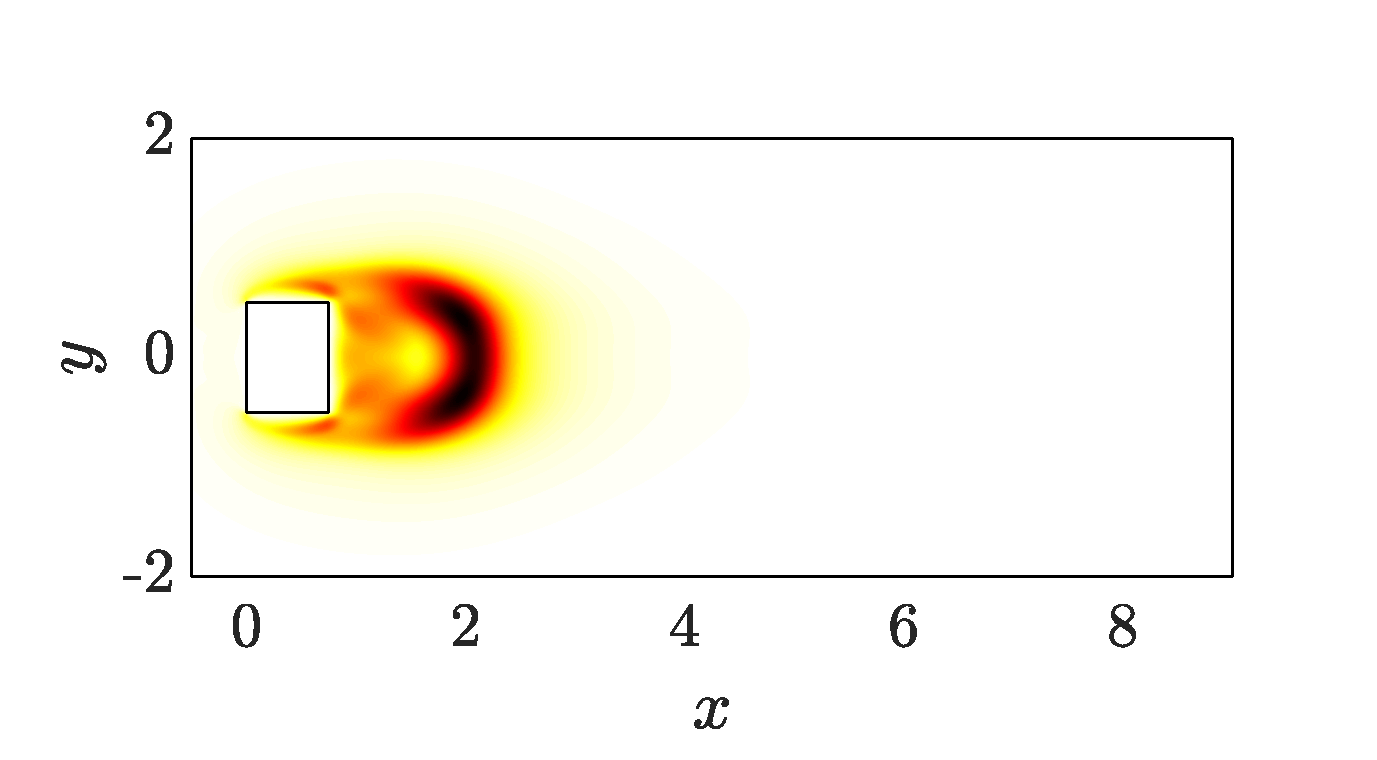
\includegraphics[width=0.49\textwidth]{./fig/AR1s/sens_AR0p75_Re140.eps}
  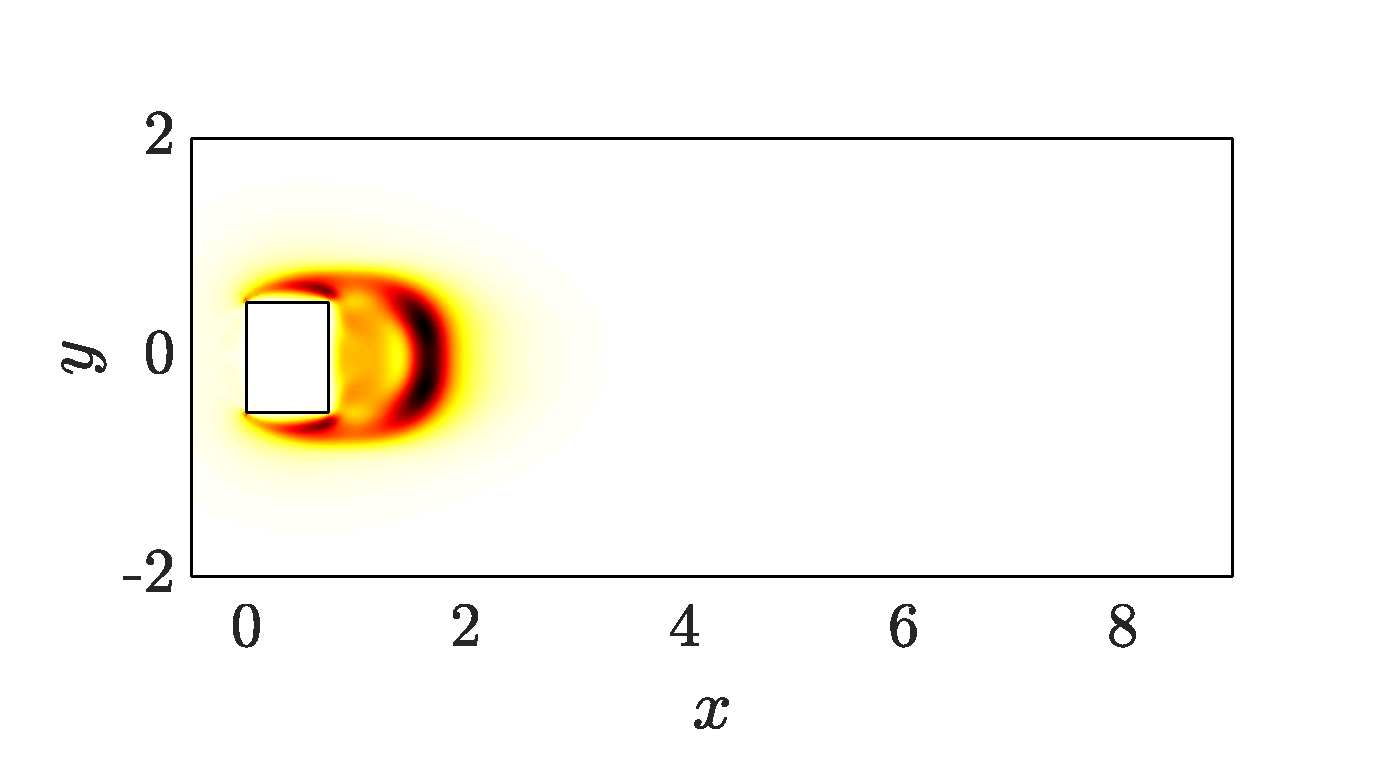
\includegraphics[width=0.49\textwidth]{./fig/AR1s/sens_AR0p75_Re230.eps} 
  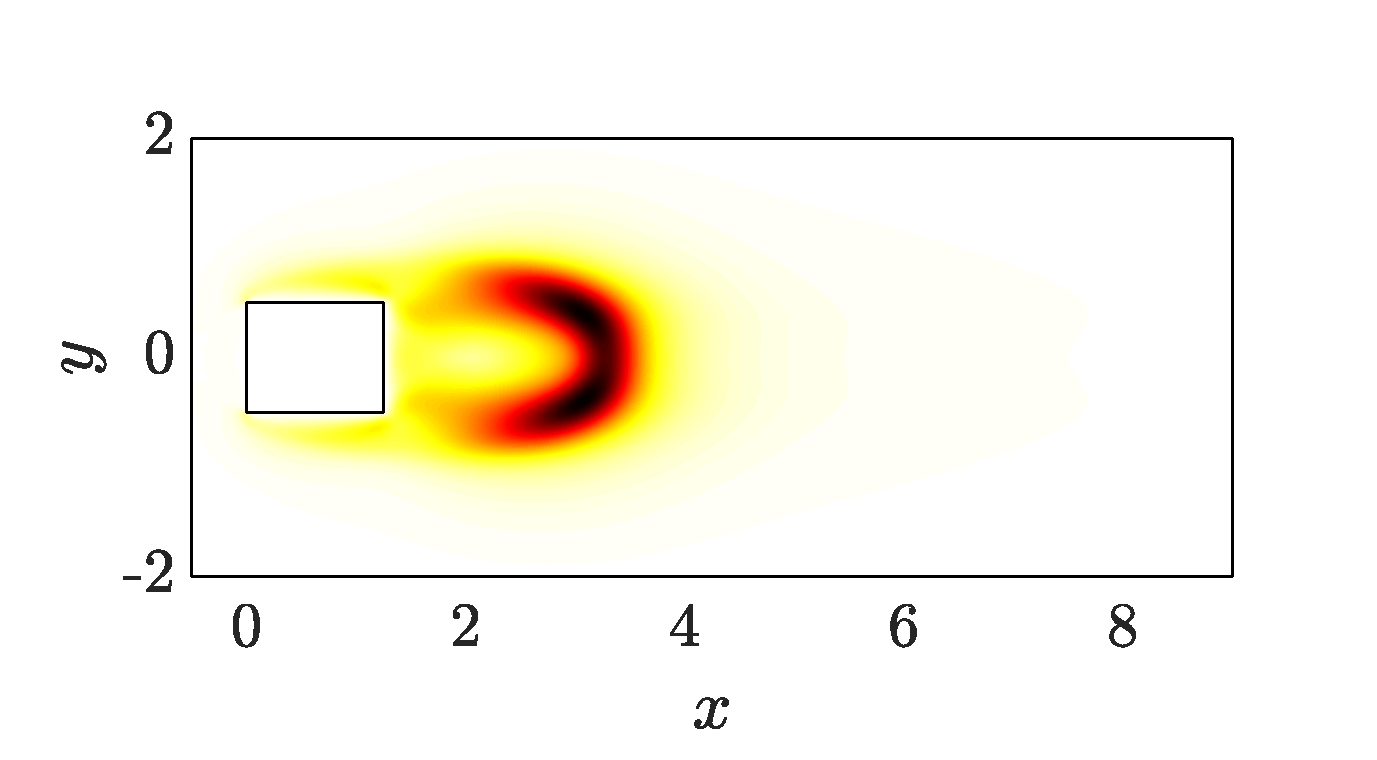
\includegraphics[width=0.49\textwidth]{./fig/AR1s/sens_AR1p25_Re140.eps}
  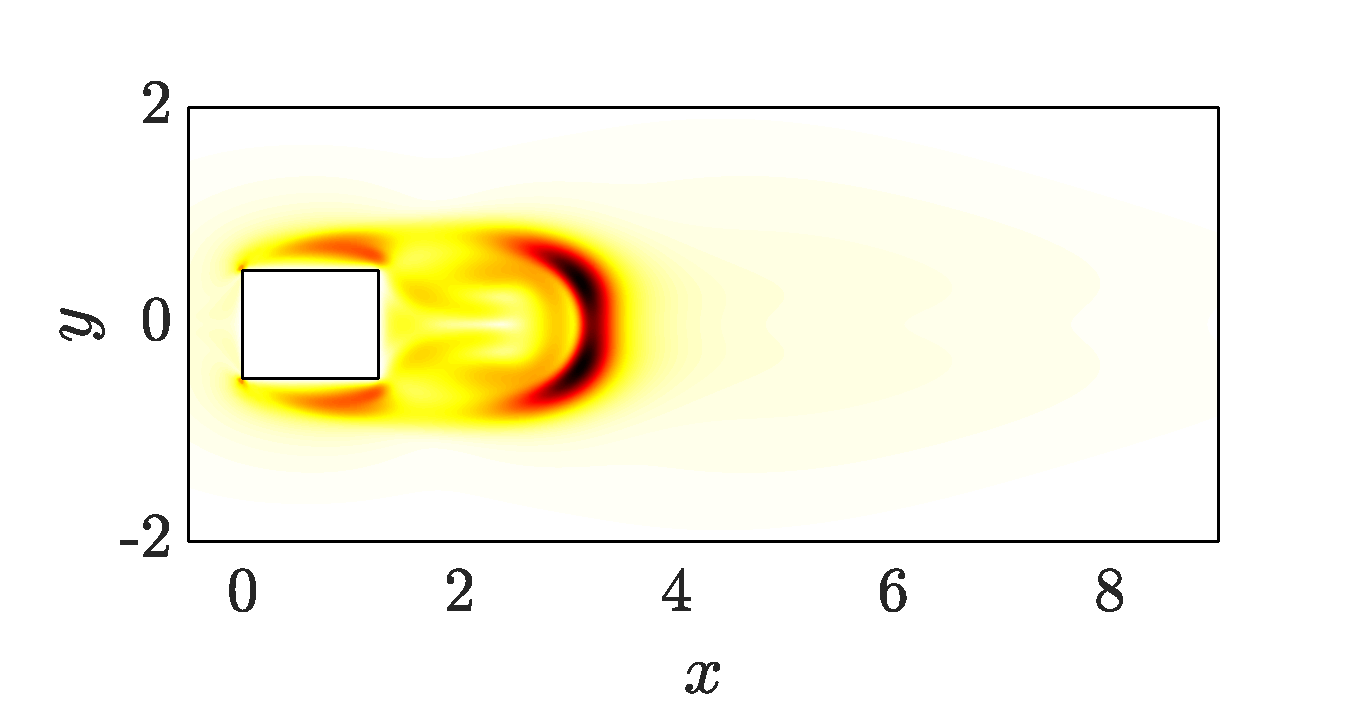
\includegraphics[width=0.49\textwidth]{./fig/AR1s/sens_AR1p25_Re230.eps}   
%  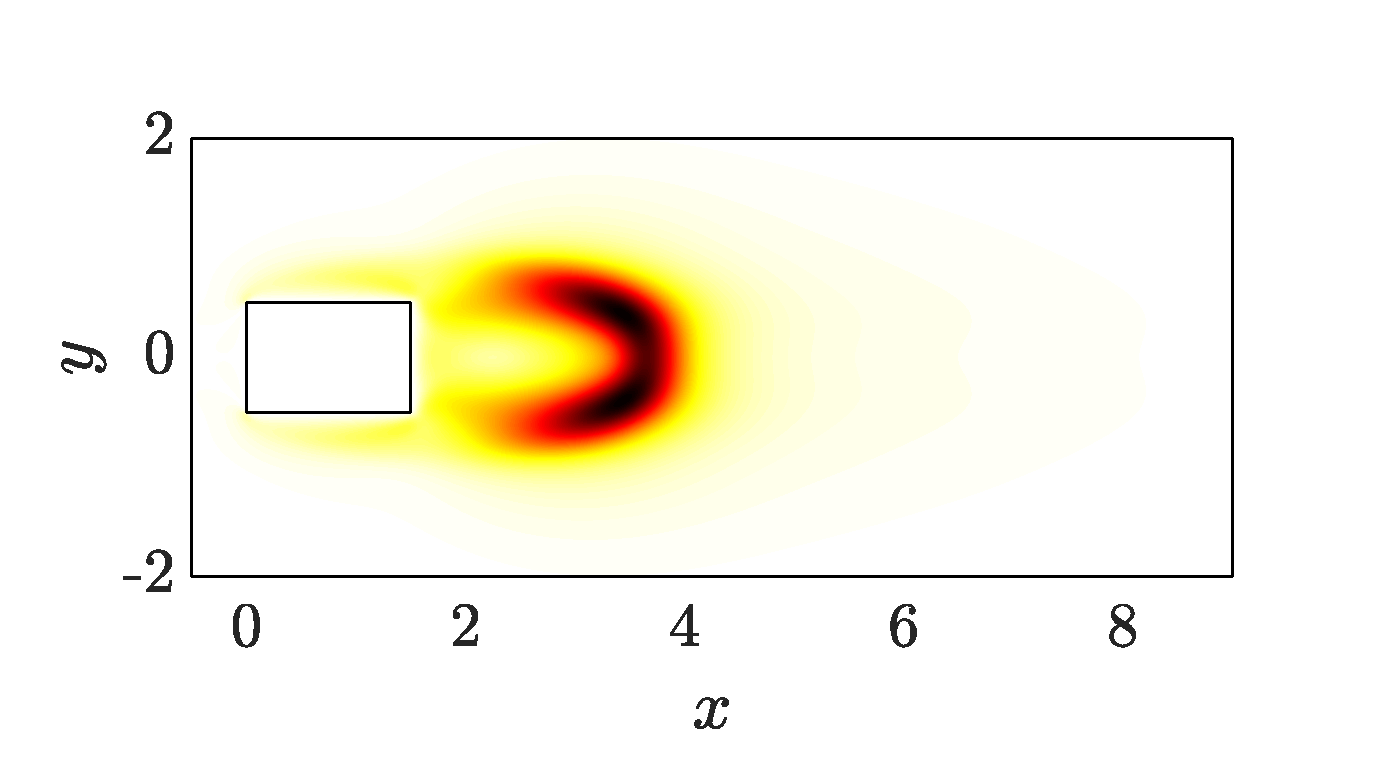
\includegraphics[width=0.49\textwidth]{./fig/AR1s/sens_AR1p5_Re140.eps}
%  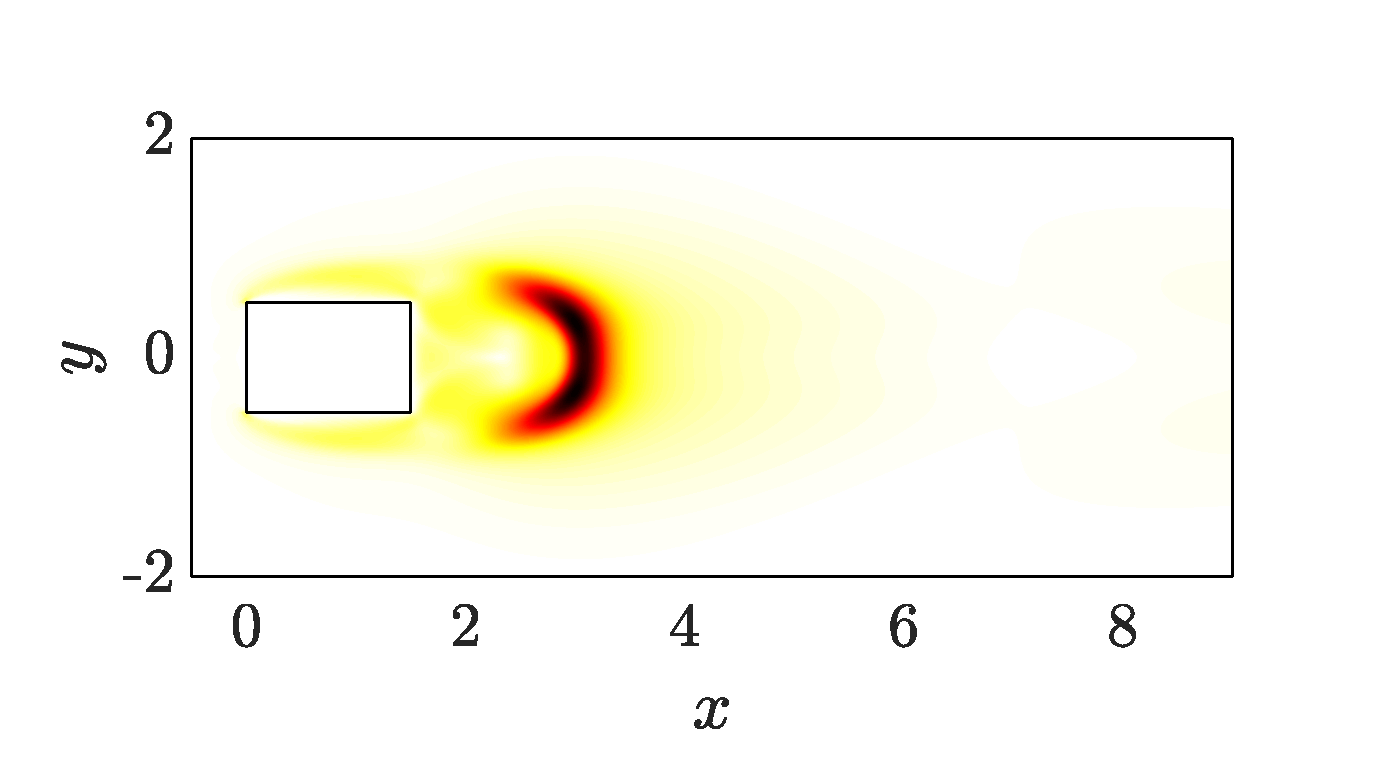
\includegraphics[width=0.49\textwidth]{./fig/AR1s/sens_AR1p5_Re230.eps} 
  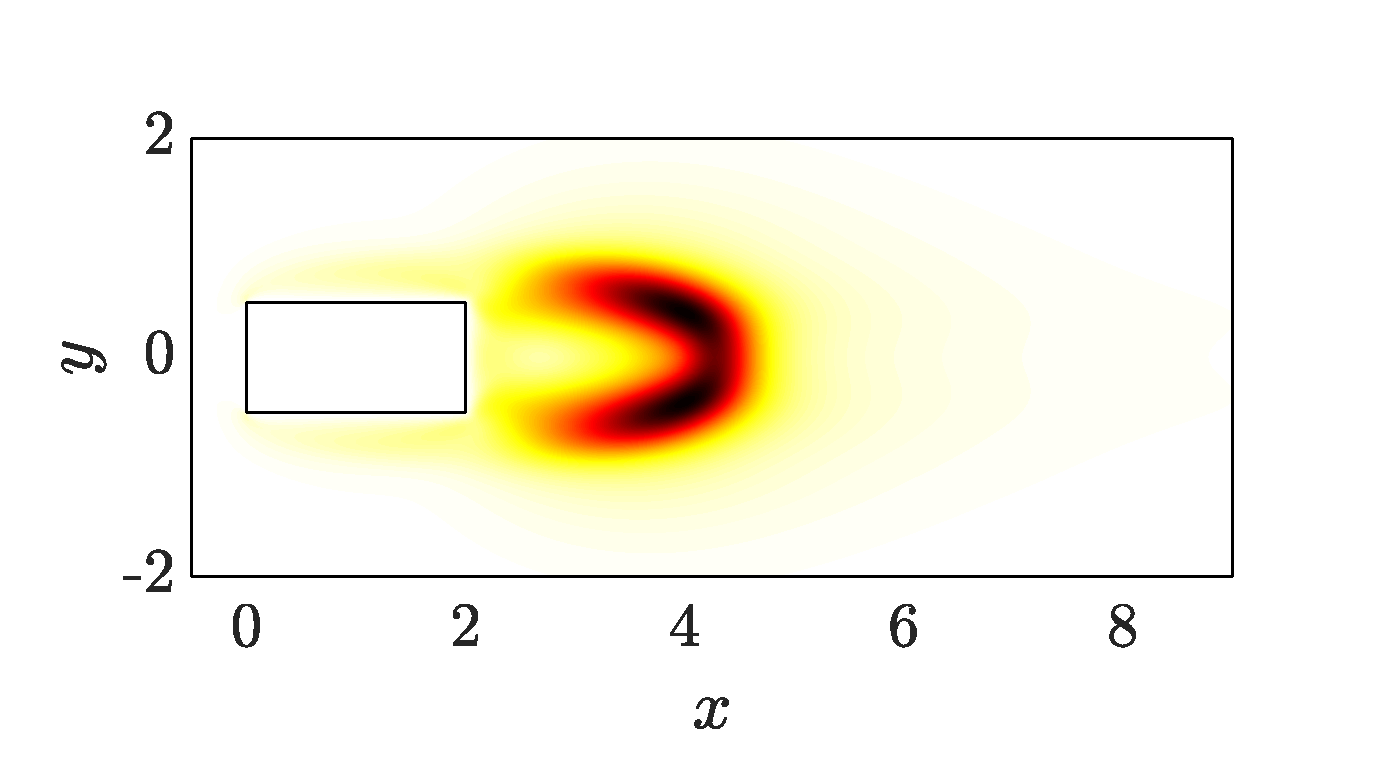
\includegraphics[width=0.49\textwidth]{./fig/AR1s/sens_AR2_Re140.eps}
  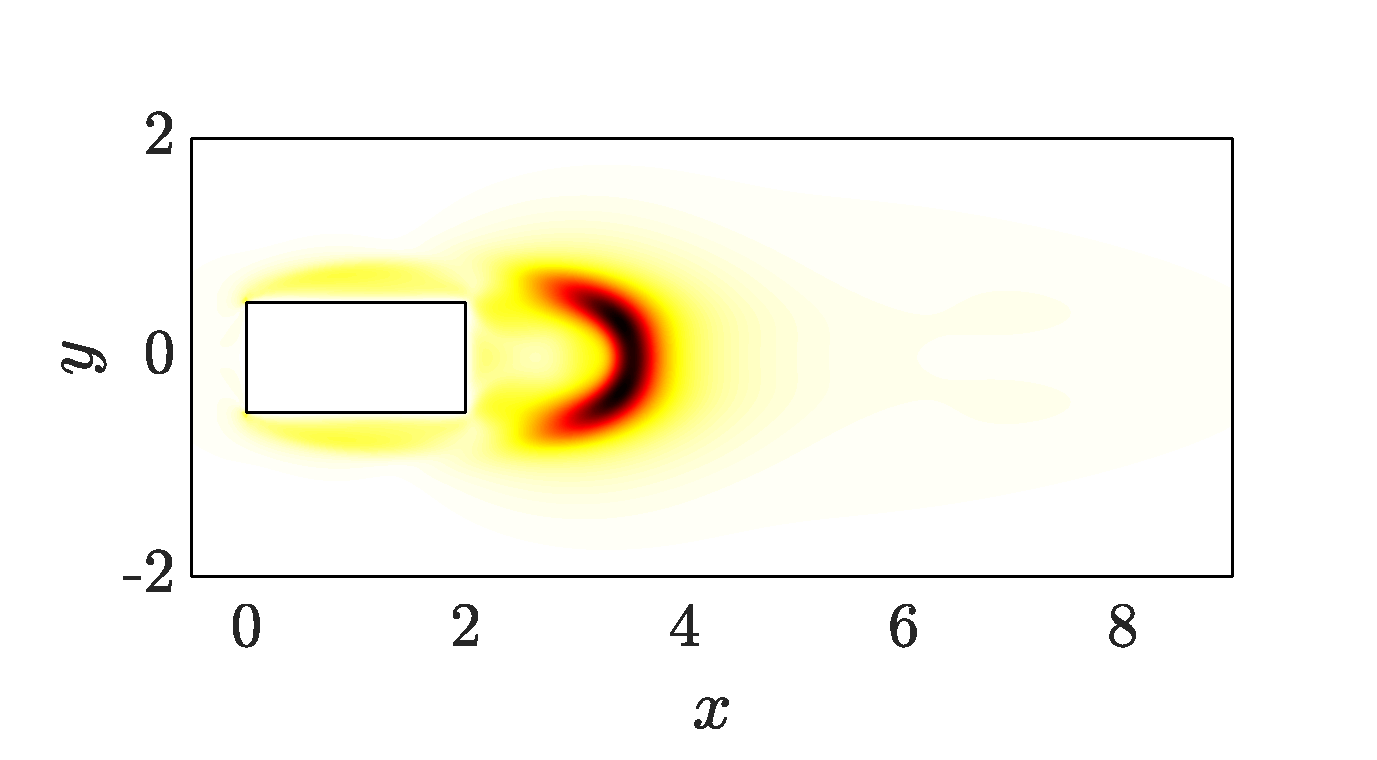
\includegraphics[width=0.49\textwidth]{./fig/AR1s/sens_AR2_Re230.eps}  
  \caption{XX SI VEDE LA DIFFERENZA. PER $\AR$ PICCOLI LO SHEDDING È DOMINATO DALLO SHEAR LAYER CHE SEPARA DAL LE. PER $\AR$ INTERMEDI, LO SHEDDING A RE BASSI È DOMINATO DAL TE SHEAR LAYER, MENTRE A RE ALTI ANCHE DAL LE SHEAR LAYER. PER $\AR$ ALTI, LO SHEDDING È DOMINATO DAL TE SHEAR LAYER PER TUTTI I RE. XX}
  \label{fig:sens-short}
\end{figure}    
%
To further investigate how flow dyanamics varies with aspect ratio $\AR$ and Reynolds number $Re$, we perform a global stability analysis of the mean flow, averaged over one shedding period. We focus on the leading eigenmode, which captures the dominant unsteady features of the flow. Similar approaches have been applied to the circular cylinder \citep{pier-2002, barkley-2006} and to elongated rectangular cylinders \citep{chiarini-quadrio-auteri-2022}.
%
The frequency of the leading eigenmode provides a good estimate of the Strouhal number observed in the nonlinear simulations across all cases, see table~\ref{tab:eigs}. Unlike the marginally stable mean flow observed for the circular cylinder \citep{barkley-2006}, our analysis yields slightly negative growth rates, suggesting a weakly damped but still dynamically relevant mean flow instability.

Figure~\ref{fig:sens-short} shows the structural sensitivity of the leading eigenmode. This quantity, introduced by \cite{giannetti-luchini-2007}, provides an upper bound on the variation of the eigenvalue resulting from a localised perturbation of the linearised Navier--Stokes operator. It corresponds to a ``force-velocity'' coupling: the feedback from a localised velocity sensor to a colocated force actuator. As such, structural sensitivity serves as an indicator of the eigenvalue's sensitivity to flow modifications and identifies the so-called wavemaker region \citep{monkewitz-etal-1993}---the core region responsible for the instability.
%
The structural sensitivity field reveals that the wavemaker is generally concentrated near the body, where the overlap of the direct and adjoint modes is largest. For longer bodies and lower $Re$, non-zero sensitivity is confined to the wake downstream of the TE, especially along the streamline bounding the mean recirculation zone. This confirms that, in these cases, the instability is driven primarily by the TE shear layers.
%
In contrast, for shorter bodies and/or higher $Re$, significant sensitivity also appears along the LE shear layers over the lateral sides. This indicates that the wavemaker extends upstream, confirming that the LE shear layers actively contribute to the vortex shedding mechanism. Overall, these results are consistent with the earlier discussion on the transition in flow topology and the corresponding changes in the shedding dynamics.


\iffalse


\begin{figure}
  \centering
  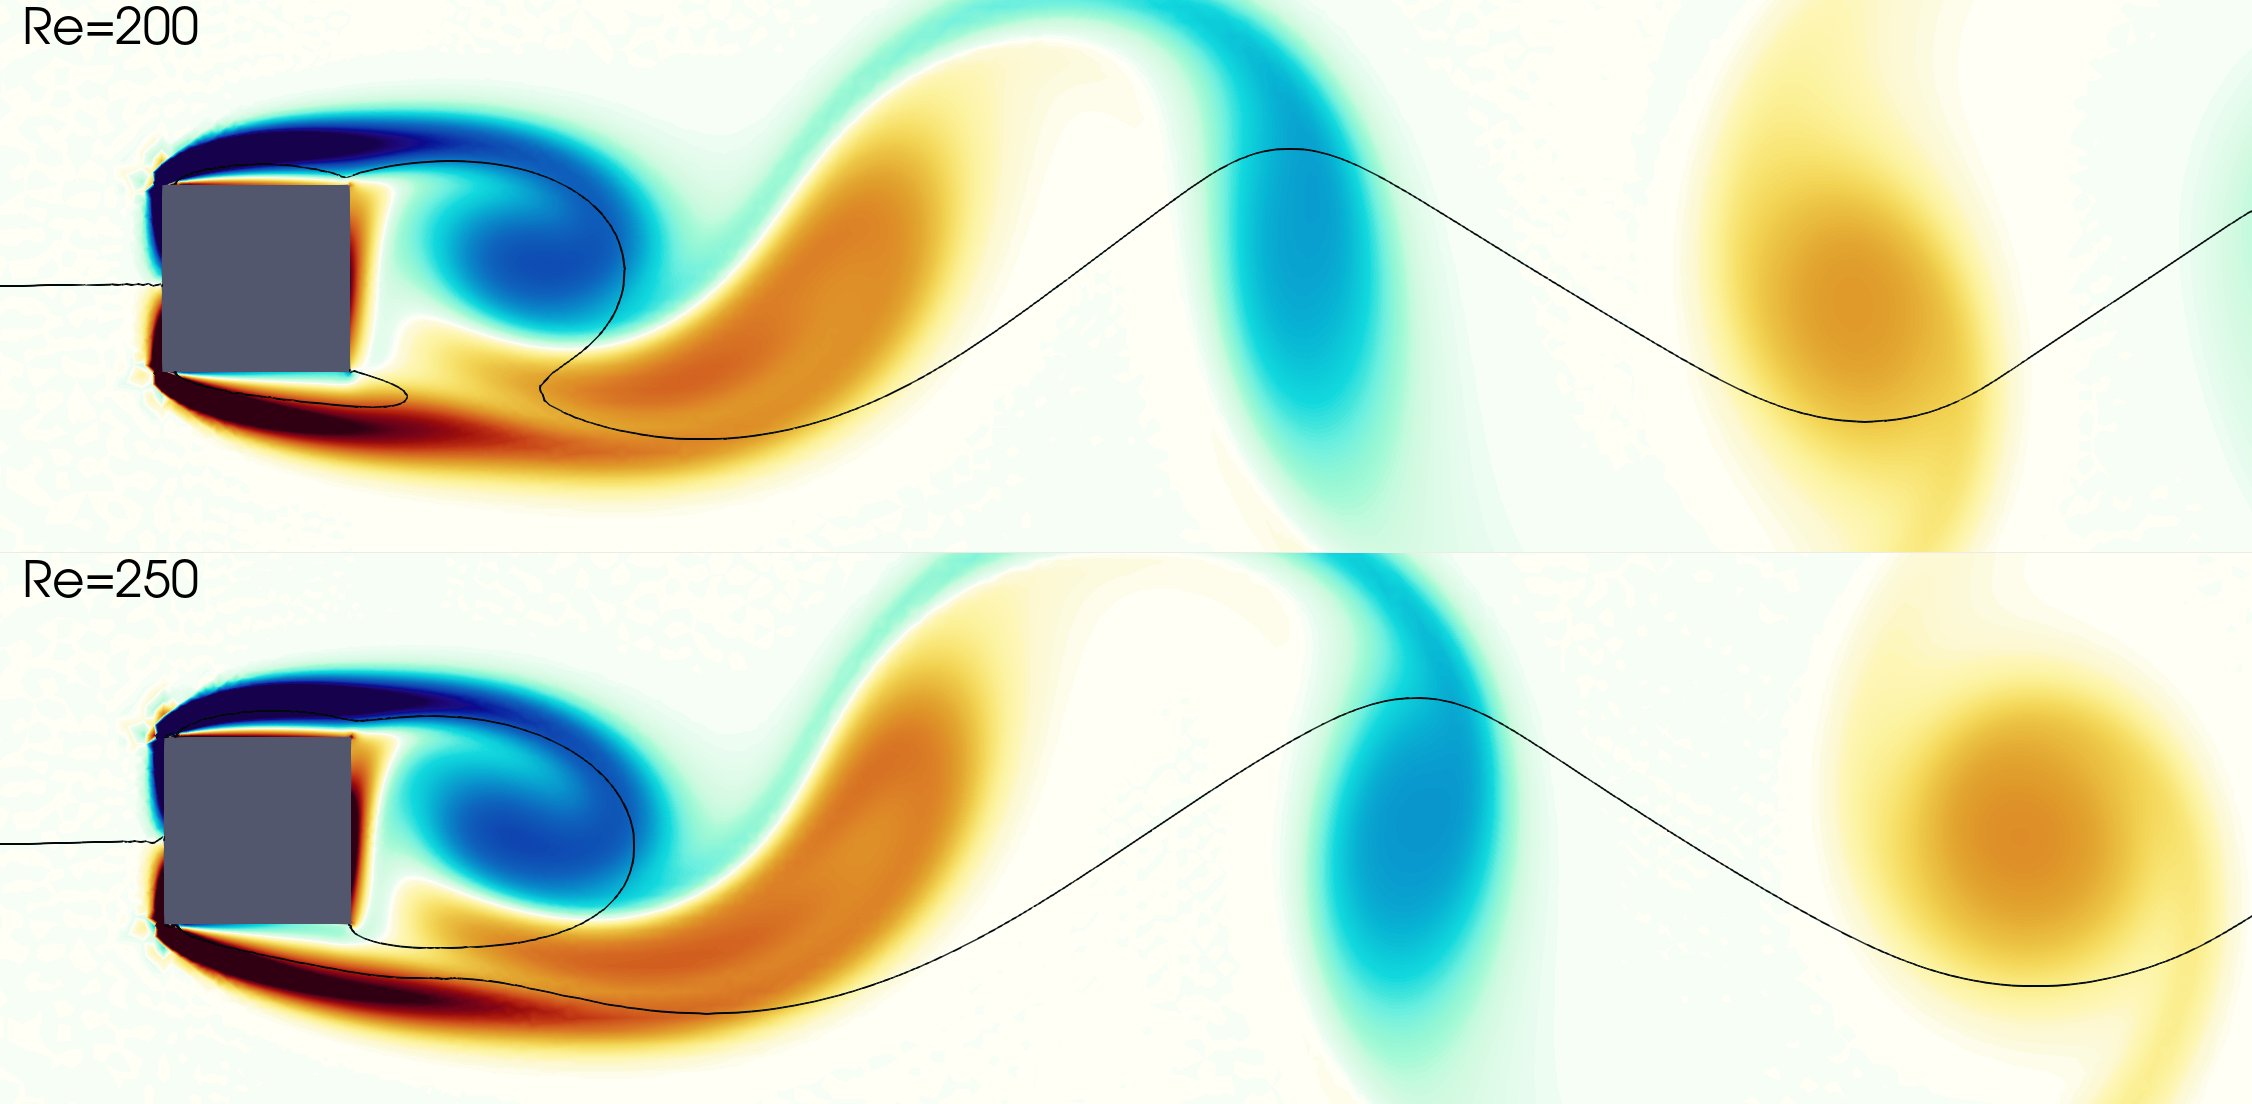
\includegraphics[width=0.49\textwidth]{./fig/AR1/snap/snap.0030.png}
  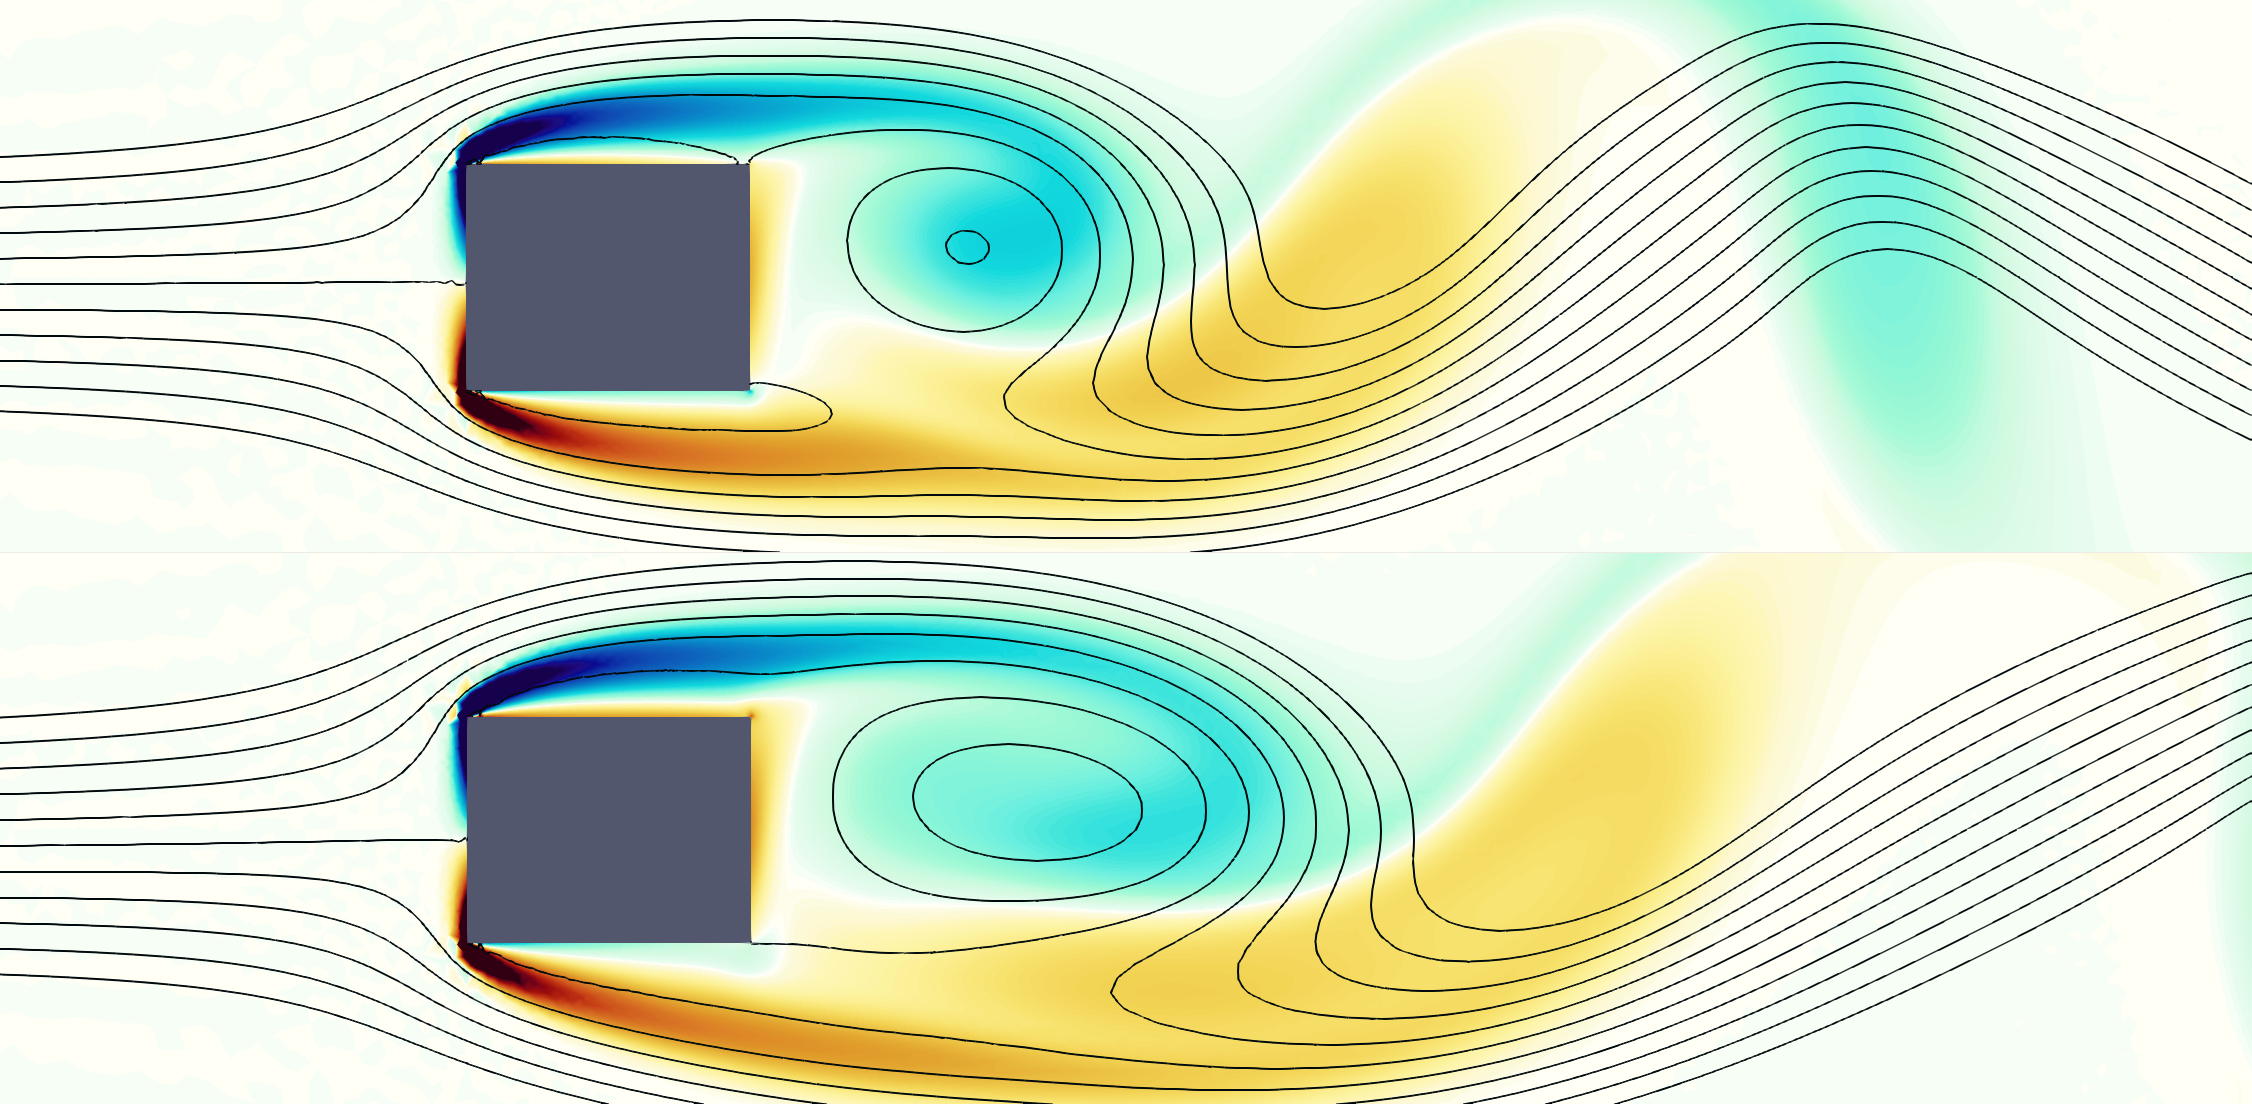
\includegraphics[width=0.49\textwidth]{./fig/AR1p25/snap/snap.0030.png}
  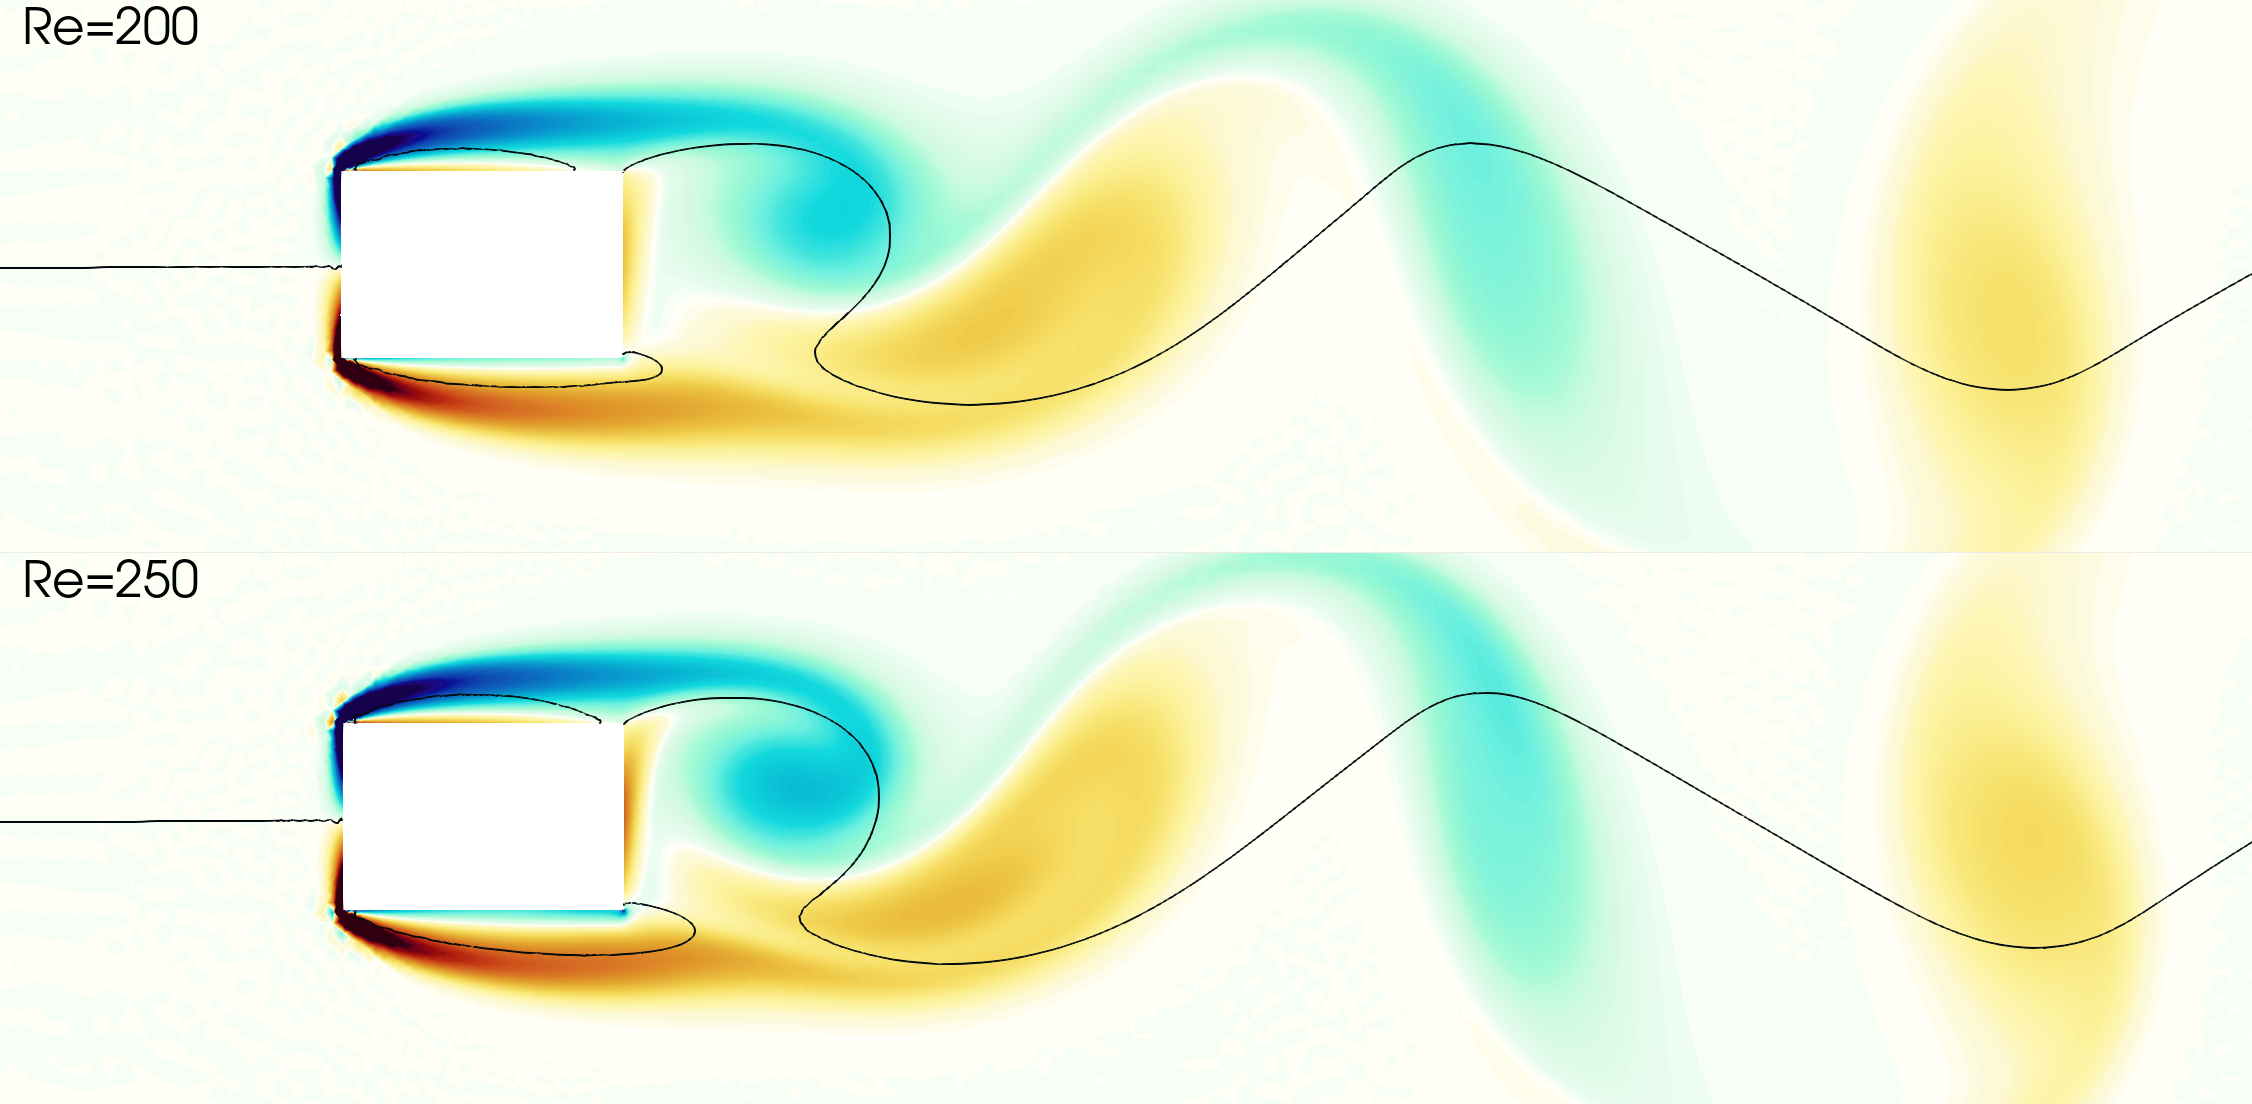
\includegraphics[width=0.49\textwidth]{./fig/AR1p5/snap/snap.0030.png}
  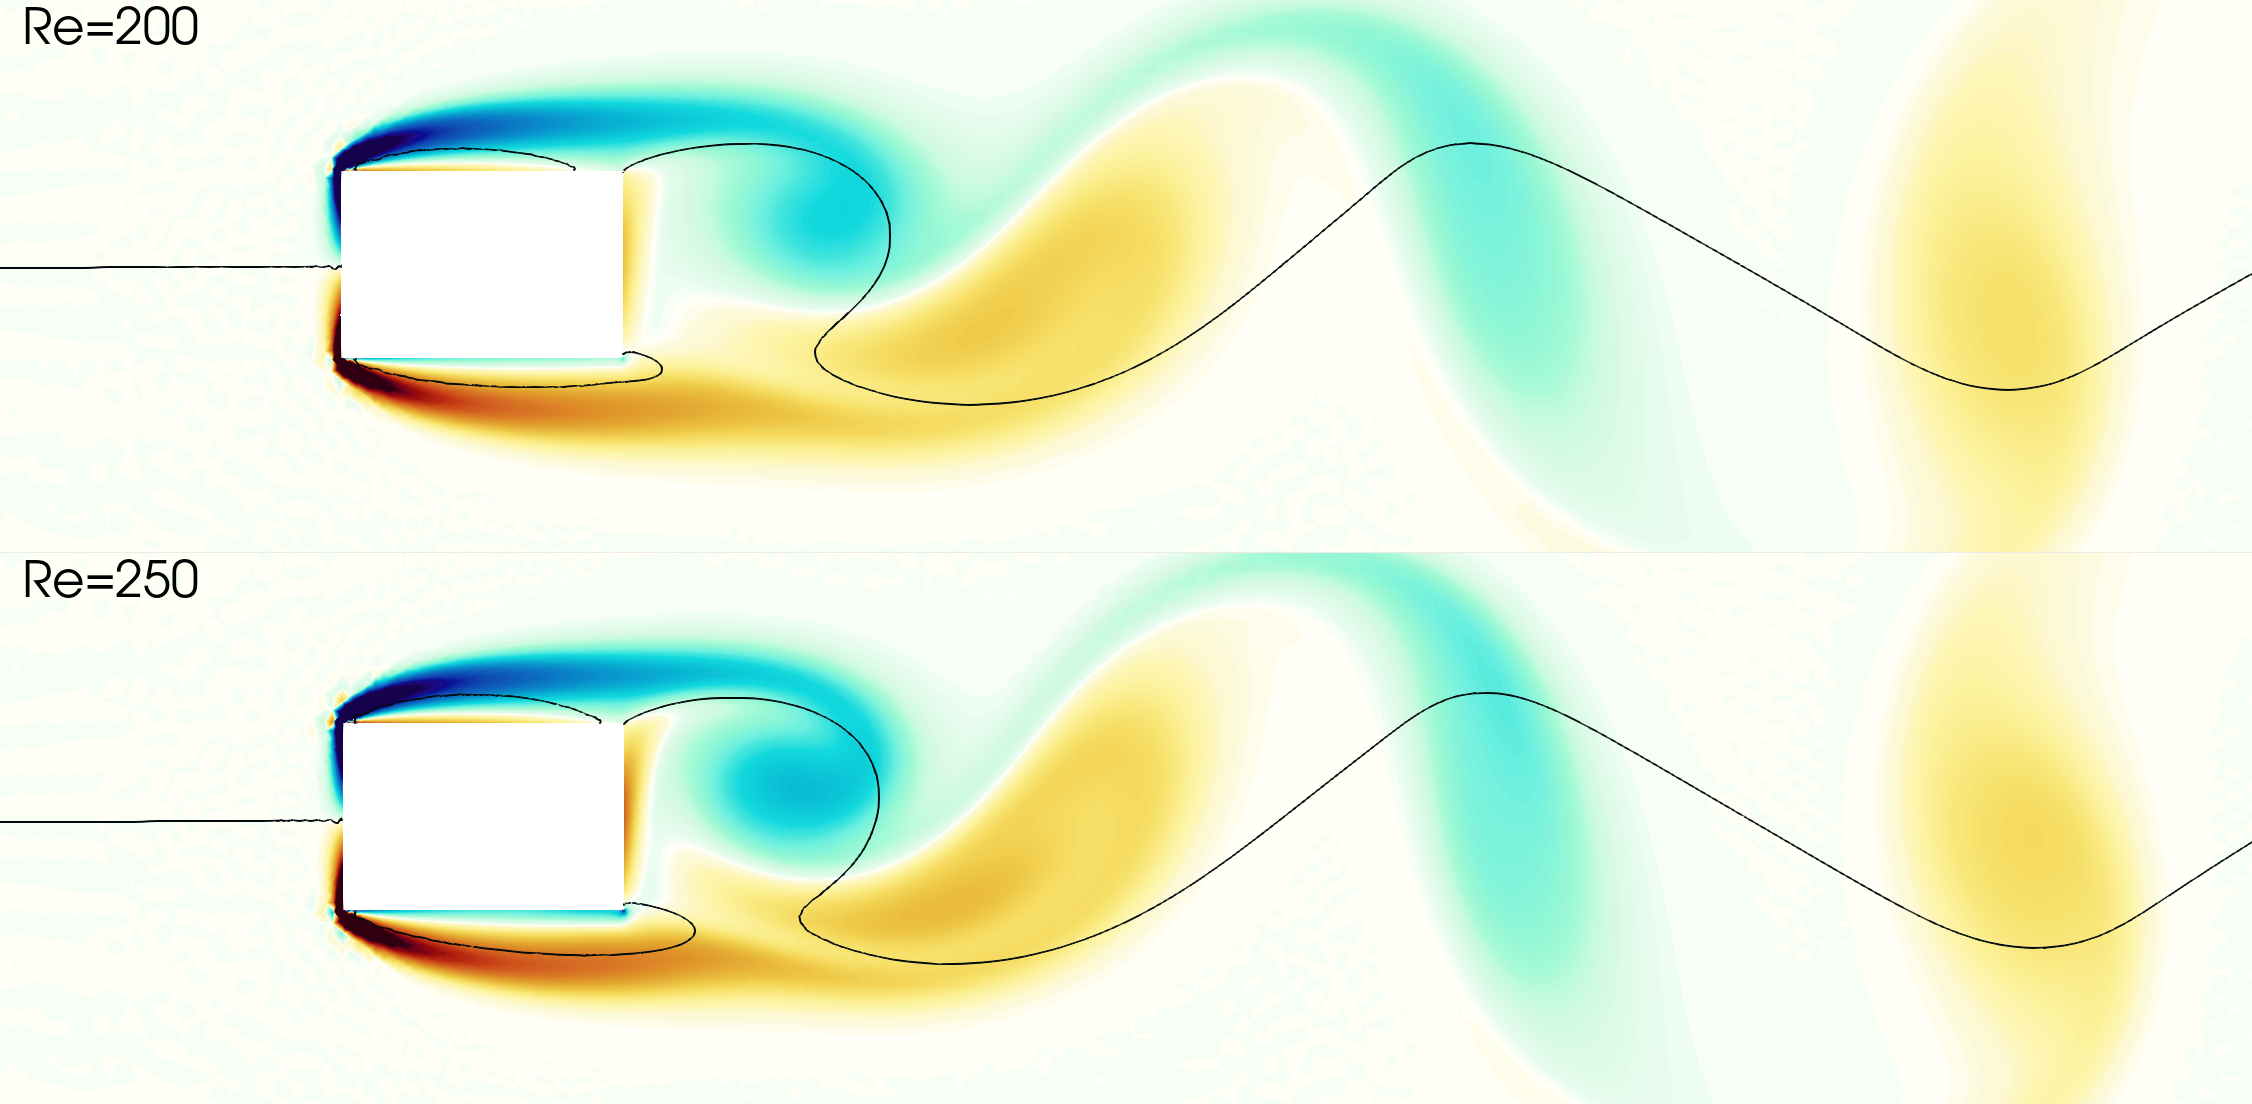
\includegraphics[width=0.49\textwidth]{./fig/AR1p5/snap/snap.0030.png}  
  \caption{Instantaneous snapshots of the base-flow vorticity for $\AR=1$ (top left), $\AR=1.25$ (top right), $\AR=1.5$ (bottom left) and $\AR=1.75$ (bottom right) at $Re=200$ (top) and $Re=250$ (bottom). For all cases the snapshots are taken at the same phase, i.e. just before the shedding of a vortex with negative vorticity in the wake. XX REPLACE $\AR=1.75$ AND ORGANISE THE FIGURE FROM TOP TO BOTTOMXX}
  \label{fig:bf-short}
\end{figure}
%
The influence of $\AR$ on the base-flow topology is shown in figure \ref{fig:bf-short}. For the smaller $\AR < 1.25$, for all considered $Re$ the flow separates at the LE and only rarely reattaches along the lateral sides of the body. In this case the vortex shedding in the wake is thus determined by the dynamics of the LE shear which is indeed active in the formation of the wake vortex. This is visualised in the figure \ref{fig:bf-short} by the streamline separating from the LE that indeed delimits the wake vortex before it is shed in the wake. By contrast, for the larger $\AR>1.25$the LE shear layer (intermittently) reattaches along the lateral sides of the body at all $Re$, and the wake dynamics is mostly determined by the TE shear layer.
For the intermediate $\AR=1.25$ the base-flow topology changes with $Re$. At the lower $Re \le 210$ the flow resembles what has been observed for longer bodies (with the LE shear layer intermittently reattaching along the lateral sides of the body), and the wake vortex shedding is driven by the TE shear layers. At the higher Reynolds numbers ($Re>210$), instead, the flow recovers the low-$\AR$ topology, with the wake dynamics being primarily driven by the LE shear layers. This is visualised in figure \ref{}, when comparing panels xx and xx and noting that the streamline separating at the LE corner reattaches for $Re=200$, but not for $Re=250$. This change of topology is explained with the fact that an increase of $Re$ leads to an increase of the angle with which the flow separates at the LE corners.

\begin{figure}
  \centering
  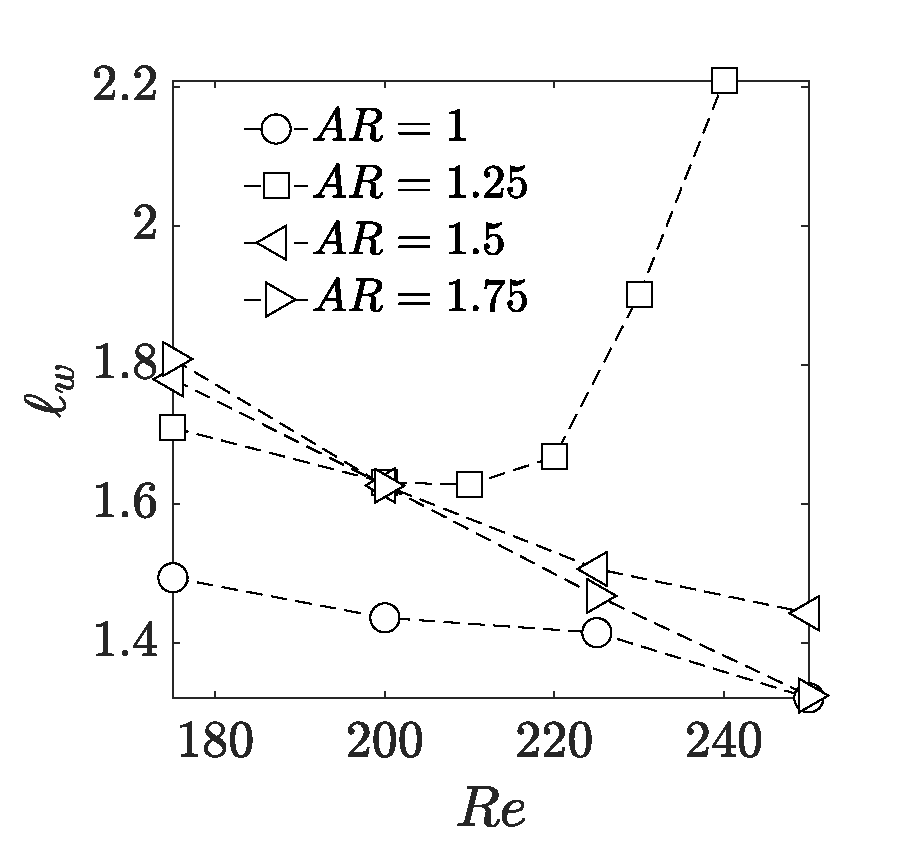
\includegraphics[width=0.32\textwidth]{./fig/AR1s/lw.eps}
  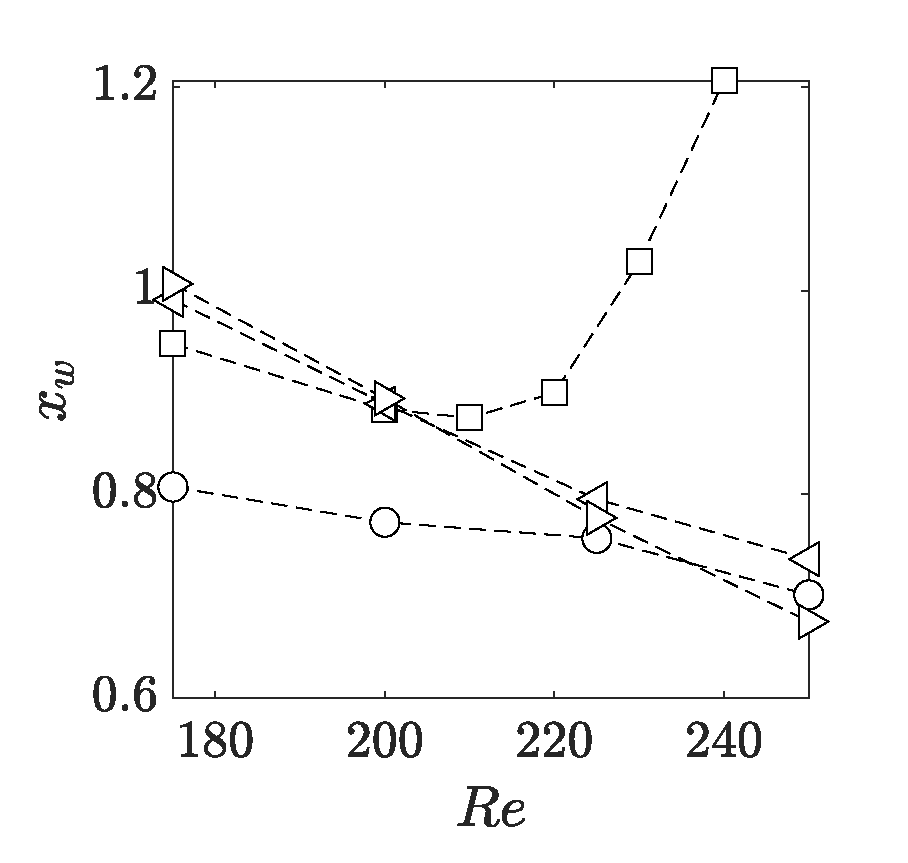
\includegraphics[width=0.32\textwidth]{./fig/AR1s/xw.eps}
  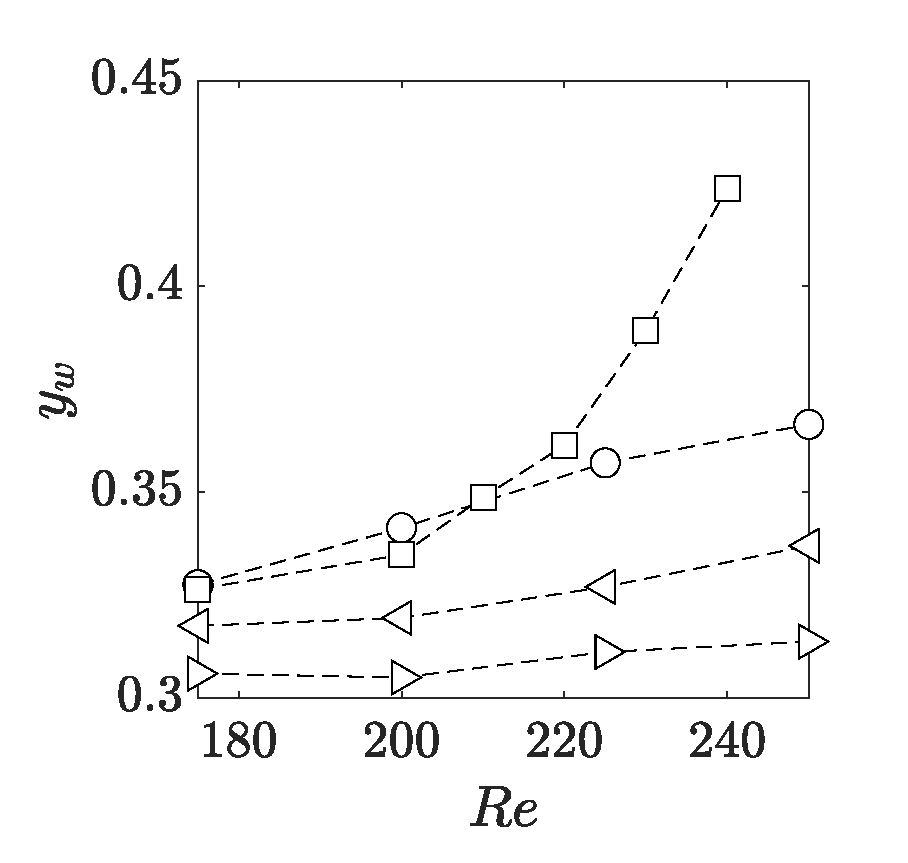
\includegraphics[width=0.32\textwidth]{./fig/AR1s/yw.eps}
  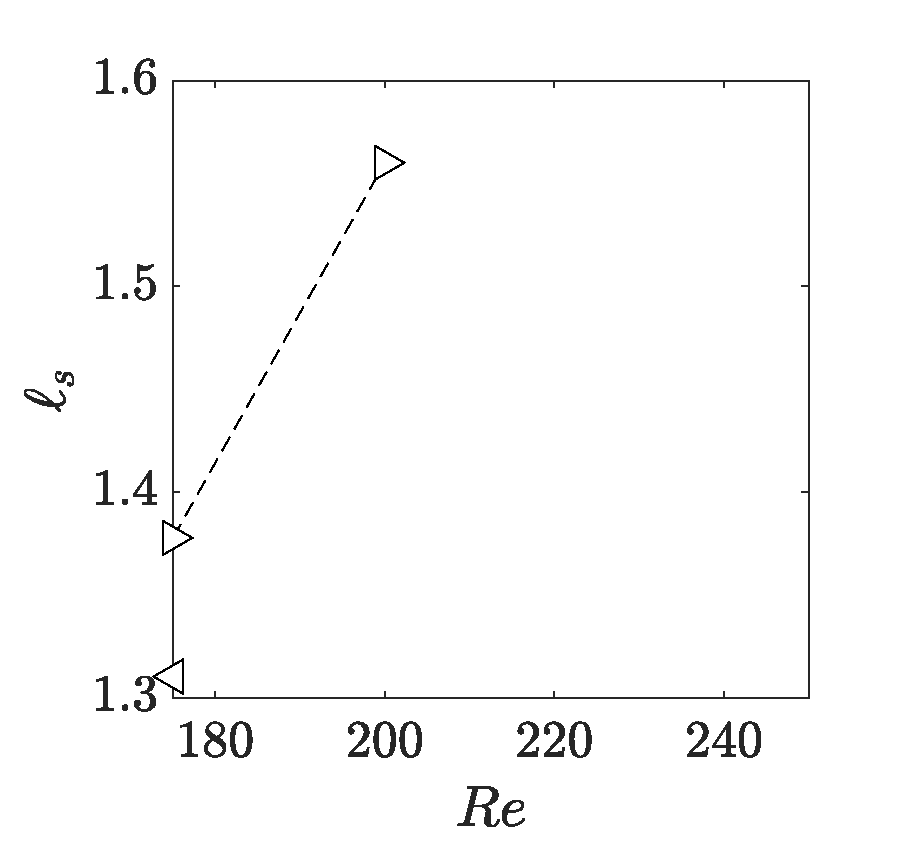
\includegraphics[width=0.32\textwidth]{./fig/AR1s/ls.eps}
  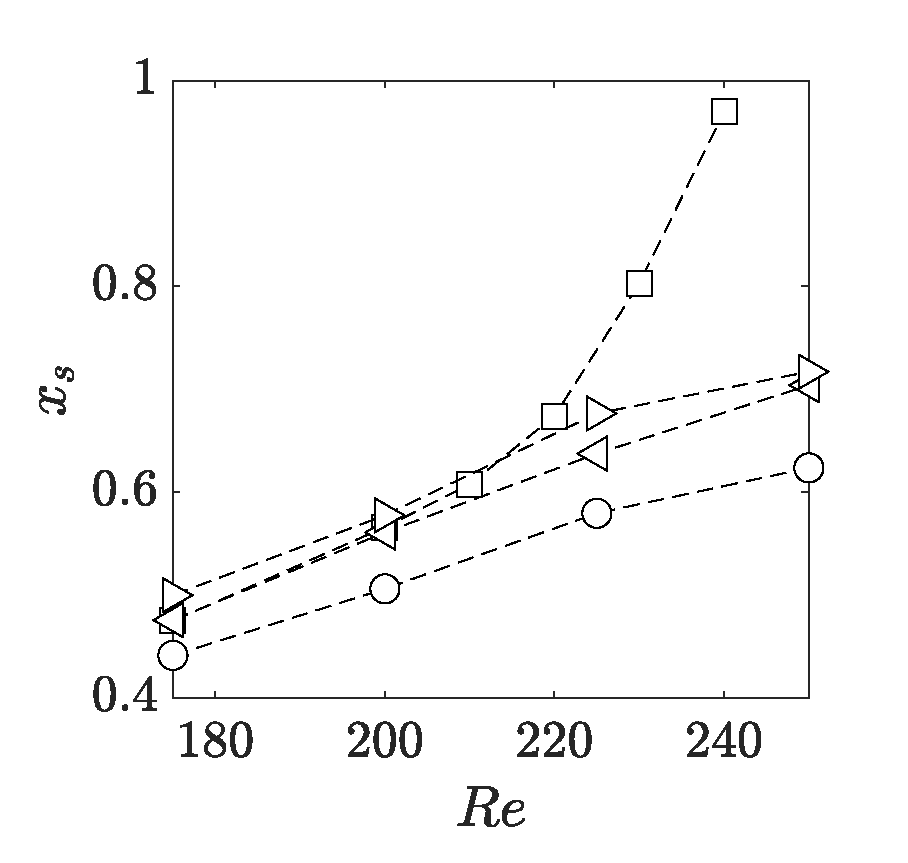
\includegraphics[width=0.32\textwidth]{./fig/AR1s/xs.eps}
  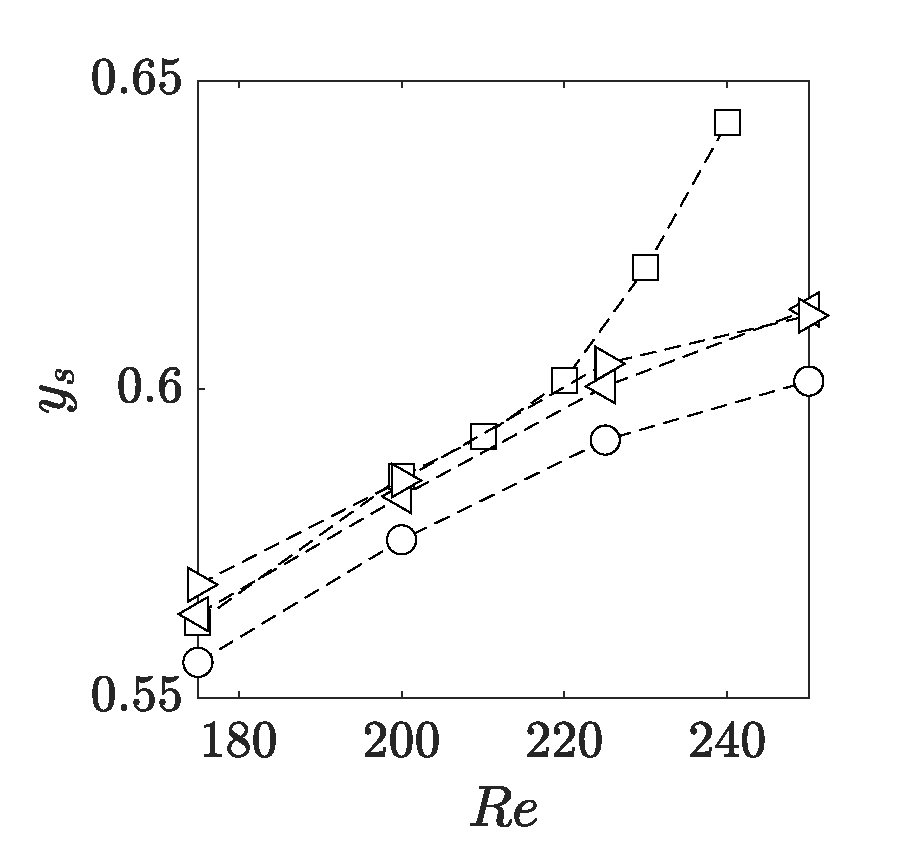
\includegraphics[width=0.32\textwidth]{./fig/AR1s/ys.eps}
  \caption{Dependence of the mean-flow properties on $\AR$ and $Re$ for $1 \le \AR \le 1.75$ and $175 \le Re \le 250$.}
  \label{fig:mf_lengths}
\end{figure}
%
We look at the mean flow averaged over one shedding period; see figure \ref{fig:mf_lengths}. For all $\AR$ an increase of $Re$ leads to an increase of the angle with which the flow separates; see dependence on $Re$ of $y_s$ and $y_w$. As a result the LE shear layers become thicker as $Re$ increases, being thus responsible for the decrease of $\ell_w$. For $\AR=1.25$ the an increase of the Reynolds number leads to a fast increase of $\ell_w$ (and $x_w$) for $Re>210$, which well correlates with the increase of the shedding period. Note that, on average, the flow reattaches along the lateral sides of the body only for $\AR \ge 1.5$ and $Re \le 200$.
% 
\begin{figure}
  \centering
  \includegraphics[width=0.49\textwidth]{./fig/AR1/LinStab/sens_Re200.eps}
  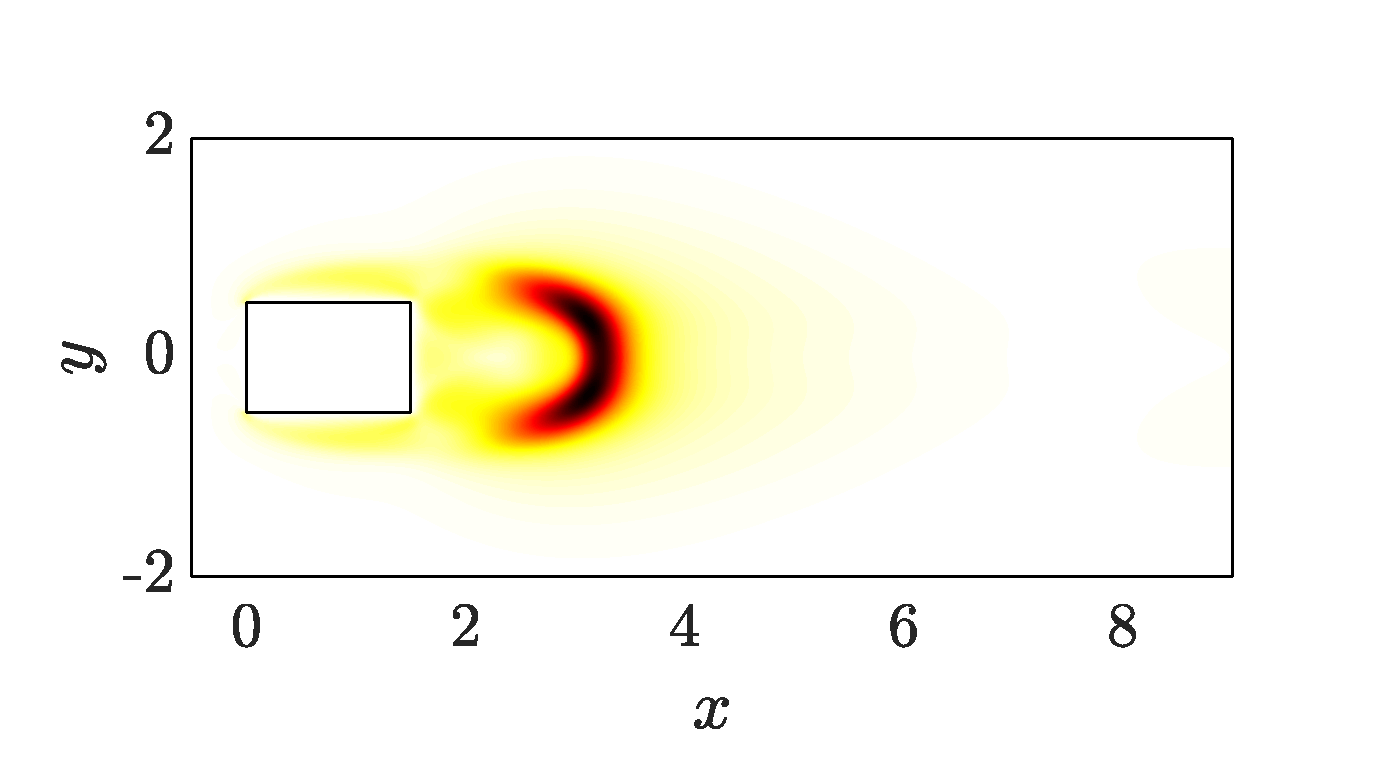
\includegraphics[width=0.49\textwidth]{./fig/AR1p5/LinStab/sens_Re200.eps}
  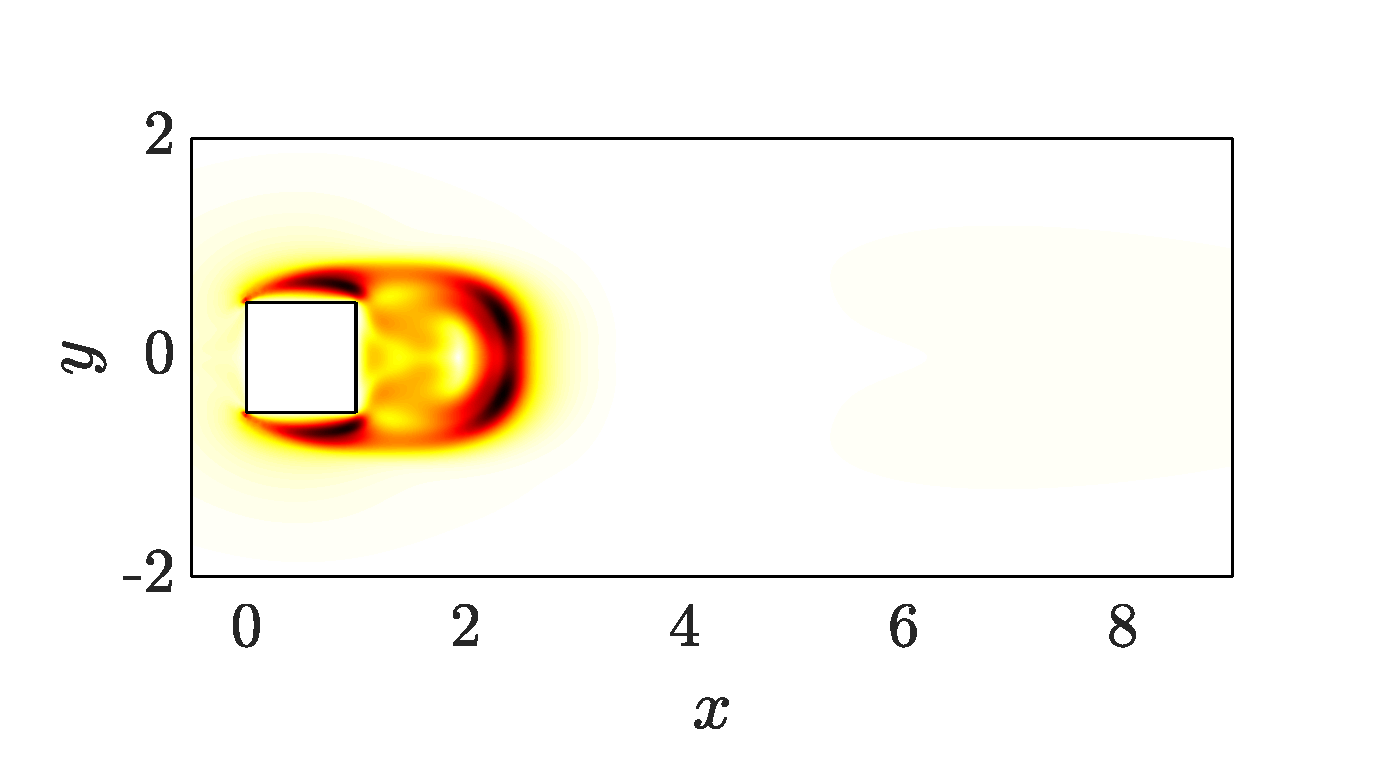
\includegraphics[width=0.49\textwidth]{./fig/AR1/LinStab/sens_Re250.eps}
  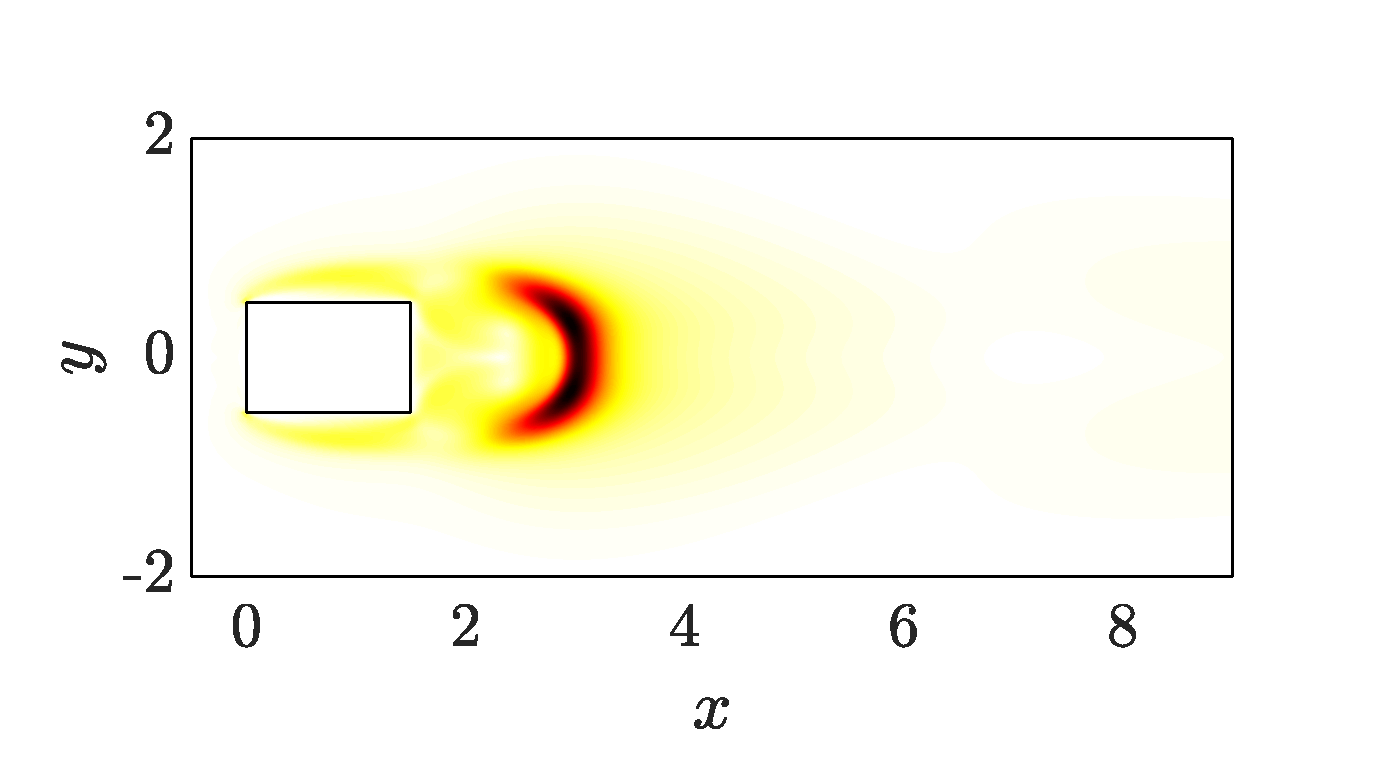
\includegraphics[width=0.49\textwidth]{./fig/AR1p5/LinStab/sens_Re250.eps}
  \includegraphics[width=0.49\textwidth]{./fig/AR1p25/LinStab/sens_Re200.eps}
  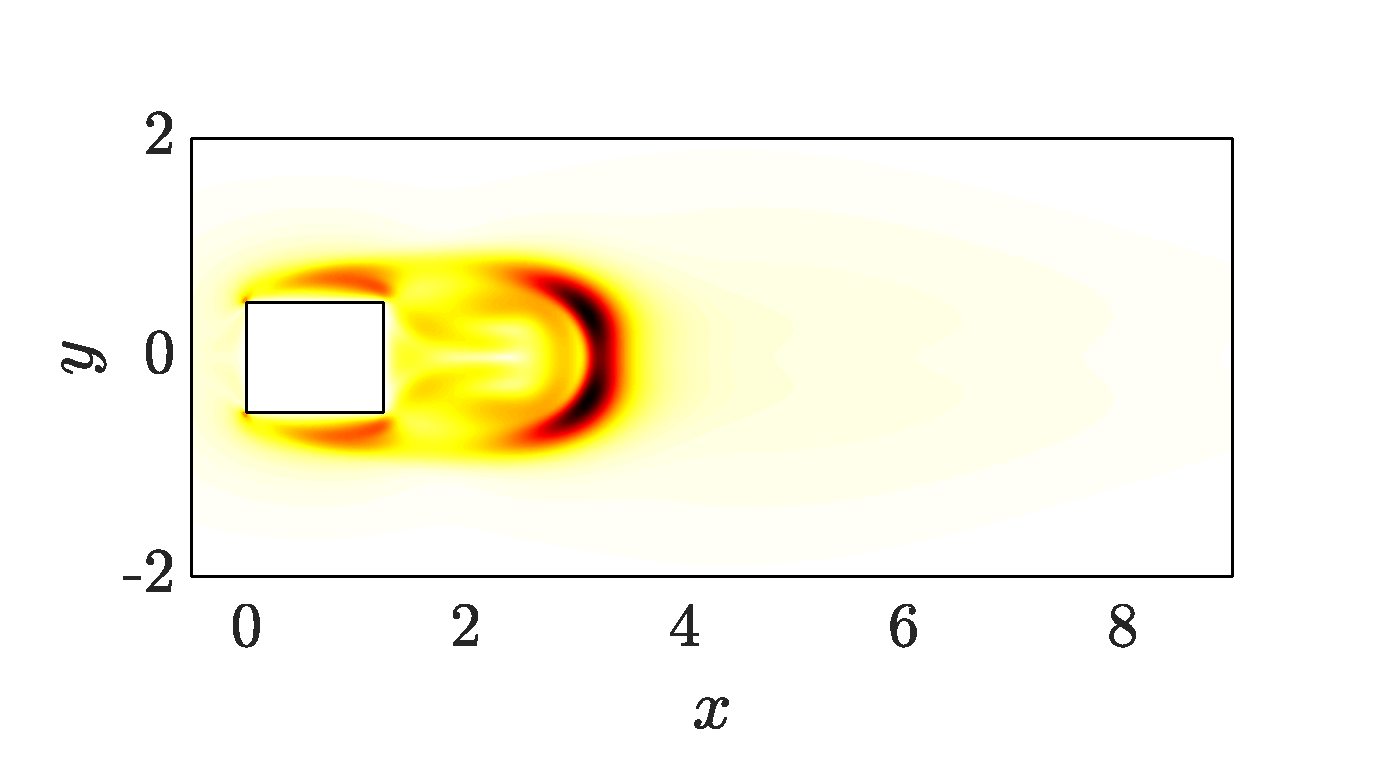
\includegraphics[width=0.49\textwidth]{./fig/AR1p25/LinStab/sens_Re230.eps}
  \caption{Linear stability analysis of the mean fow for $\AR=1$ and $Re=200$ (top left), $\AR=1.5$ and $Re=200$ (top right), $\AR=1$ and $Re=250$ (centre left), $\AR=1.5$ and $Re=250$ (centre right) $\AR=1.25$ and $Re=200$ (bottom left) and $\AR=1.25$ and $Re=230$ (bottom right).}
  \label{fig:mf_sens}
\end{figure}
%
To further highlight the change of the flow topology with $\AR$ and $Re$, we perform a global stability analysis of the mean flow averaged over one shedding period. The focus in on the leading eigenmode, which is representative of the unsteady phenomena of the flow. For a similar approach see for example \cite{pier-2002,barkley-2006} for the circular cylinder and \cite{chiarini-quadrio-auteri-2022} for rectangular cylinders. 

The frequency of the leading eigenmode predicts fairly well the Strouhal number observed in the nonlinear simulations for all cases, with a maximum difference of $xx\%$. Unlike the case of the circular cylinder, which is marignally stably \citep{barkley-2006}, the present mean flow stability analysis leads to a slightly negative growth rate. Figure \ref{fig:mf_sens}, shows the structural sensitivity of the leading mode. The structural sensitivity was introduced by \cite{giannetti-luchini-2007} as an upper bound for the eigenvalue variation induced by a specific perturbation of the linearised Navier--Stokes operator, namely a `force-velocity coupling' representing feedback from a localised velocity sensor to a localised force actuator at the same location. In this sense, the structural sensitivity in as indicator of the eigenvalue sensitivity and identifies the wavemaker \citep{monkewitz-etal-1993}. The structural sensitivity identifies the flow region where structural modifications of the stability problem produce the strongest drift of the leading eigenvalue and indentifies the so-called wavemaker. The largest values of the sensitivity occur near the cylinders, as the product of the adjoint and direct modes is small in the remaining part of the domain. For longer bodies and smaller $Re$ non null values are observed only in the wake behind the TE along the streamline delimiting the mean recirculating region. The core of the instability responsible for the TE vortex shedding is located downstream the TE. For shorter bodies and/or larger $Re$ the structural sensitivity is non negligible also along the LE shear layers over the lateral sides of the cylinder. Accordingly, in these cases the wavemaker extends to the LE shear layers, as they play a role inthe wave vortex shedding dyanmics.
\fi

\subsection{The bifurcations}

\begin{figure}
  \centering
  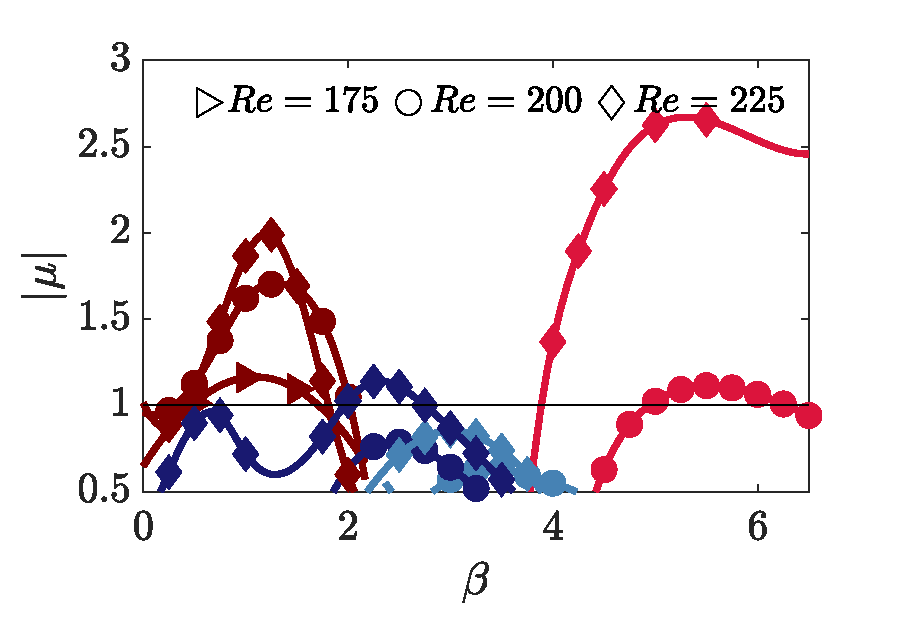
\includegraphics[width=0.49\textwidth]{./fig/AR1/neutralb.eps}
  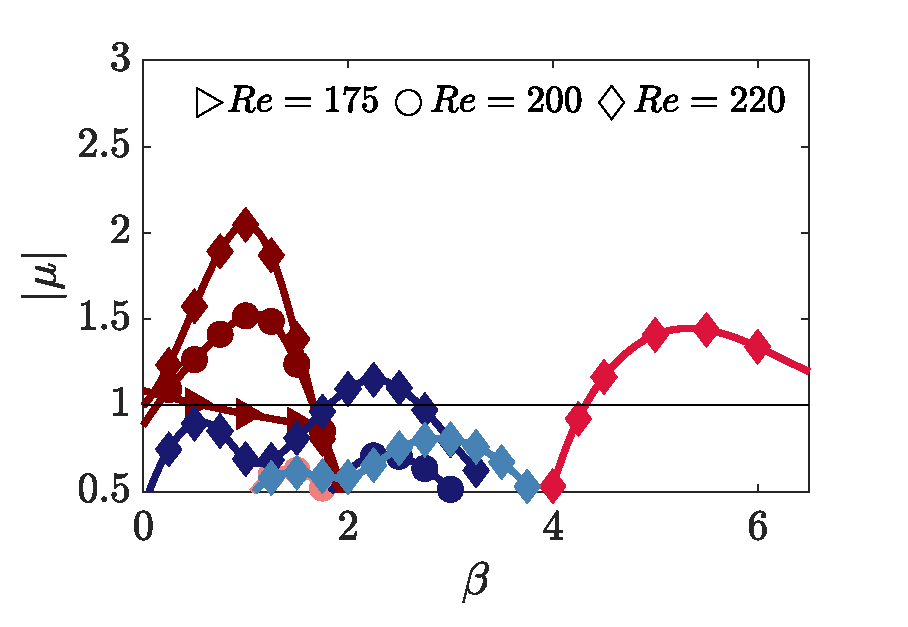
\includegraphics[width=0.49\textwidth]{./fig/AR1p25/neutralb.eps}  
  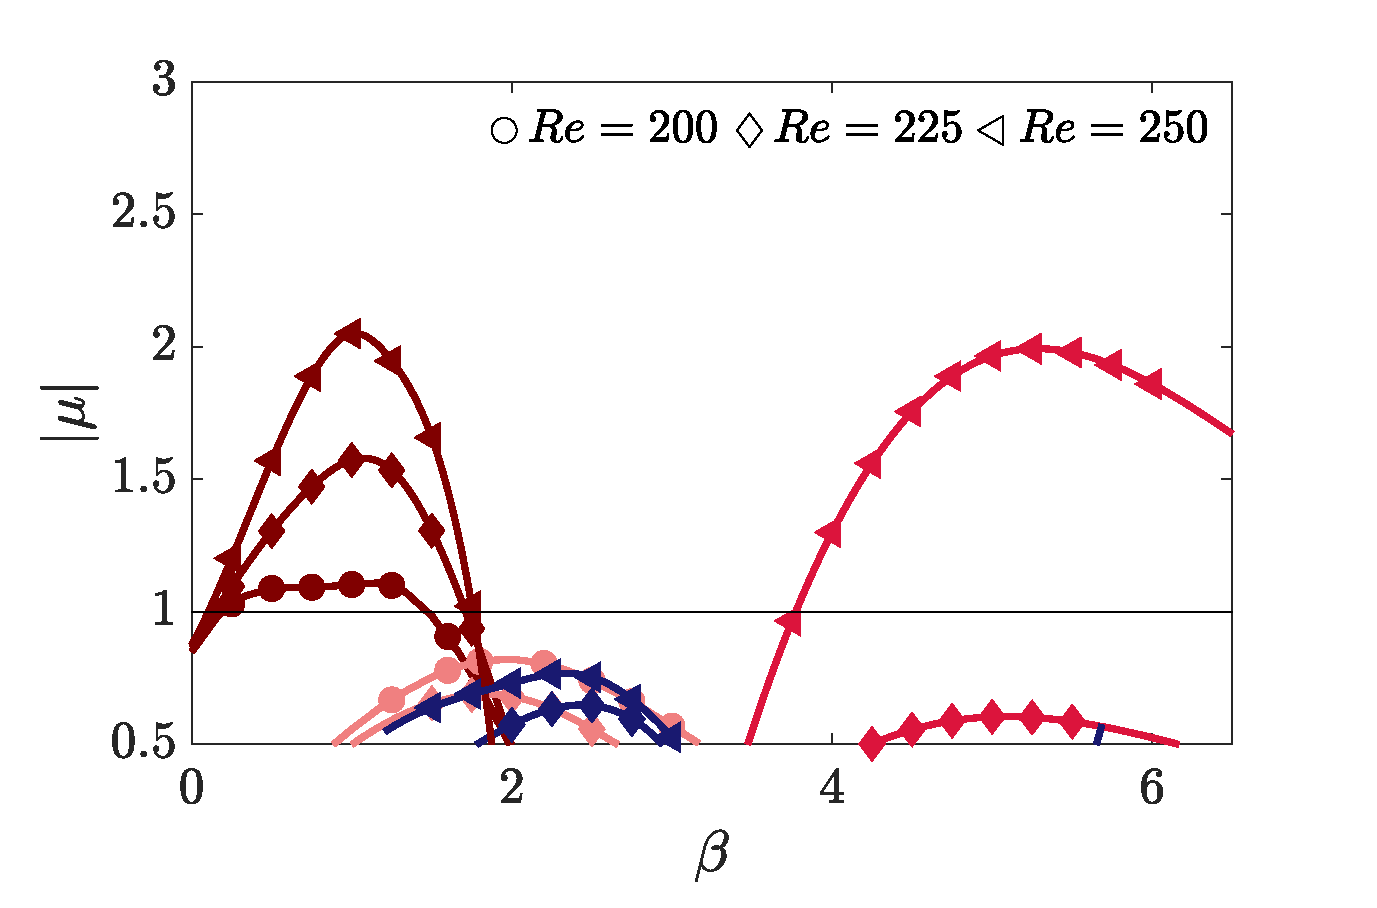
\includegraphics[width=0.49\textwidth]{./fig/AR1p5/neutralb.eps}    
  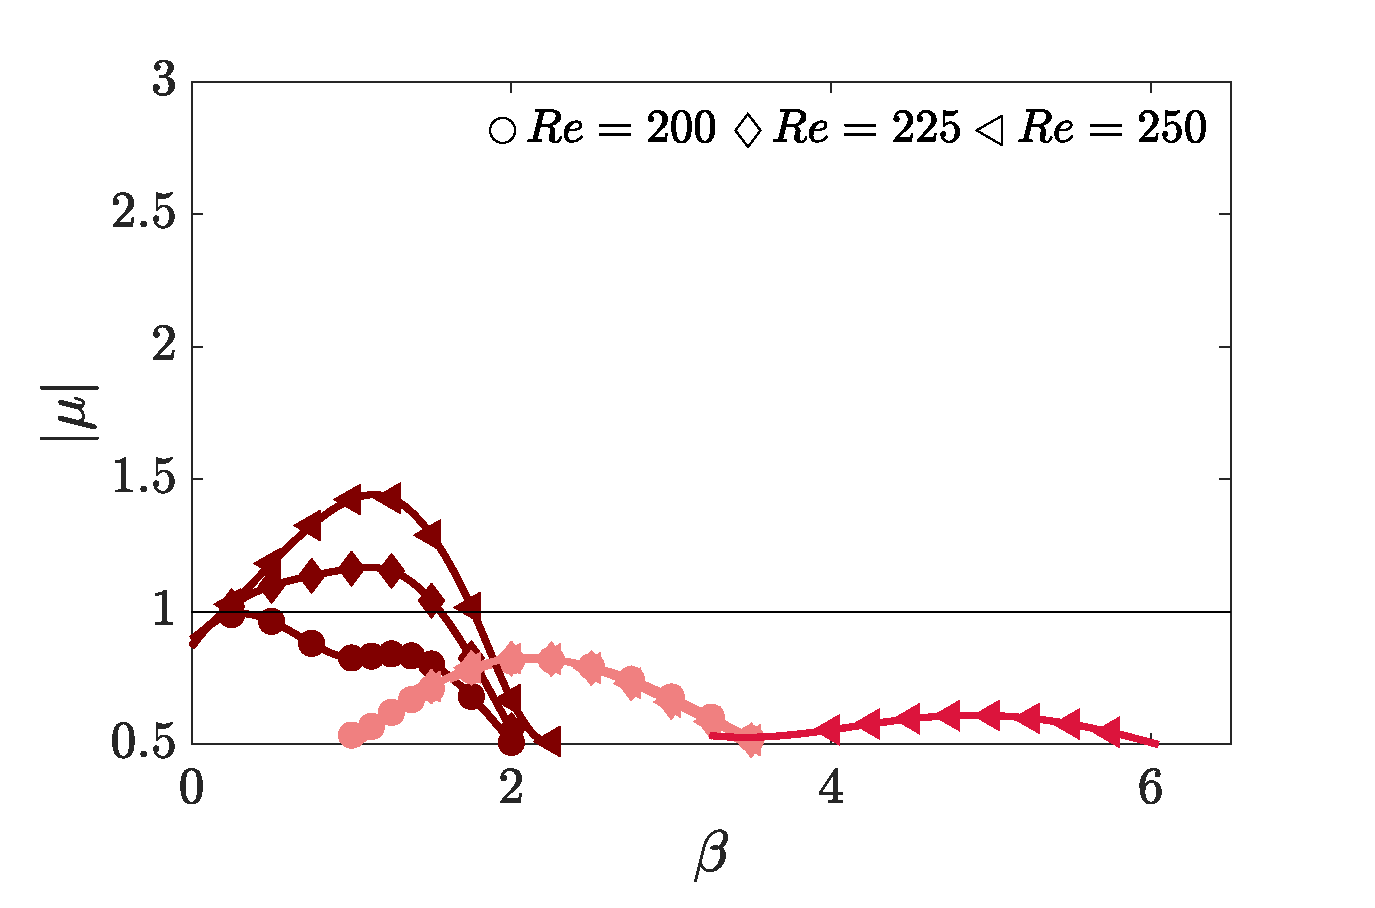
\includegraphics[width=0.49\textwidth]{./fig/AR1p75/neutralb.eps}       
  \caption{Multipliers for $\AR=1$ (top left), $\AR=1.25$ (top right), $\AR=1.5$ (bottom left) and $\AR=1.75$ (bottom right) for different $Re$. The dark red line refers to mode $A$, the light blue line to mode $C$, the light red to mode $B$, the dark blue lines to mode $QP$, the light blue line refers to mode $B'$, and pink lines mode $C$. Mode $B'$ has the same spatio-temporal symmetry of mode $B$, but its characteristic wavelength is much smaller, being similar to that of mode $A$. This mode resembles that found for elongated bodies with elliptic leading edge by \cite{ryan-etal-2005}. XX ADD $\AR=2$ e $\AR=2.5$ XX}
  \label{fig:mult_AR1_AR1p75}
\end{figure}
%
\begin{figure}
  \centering
  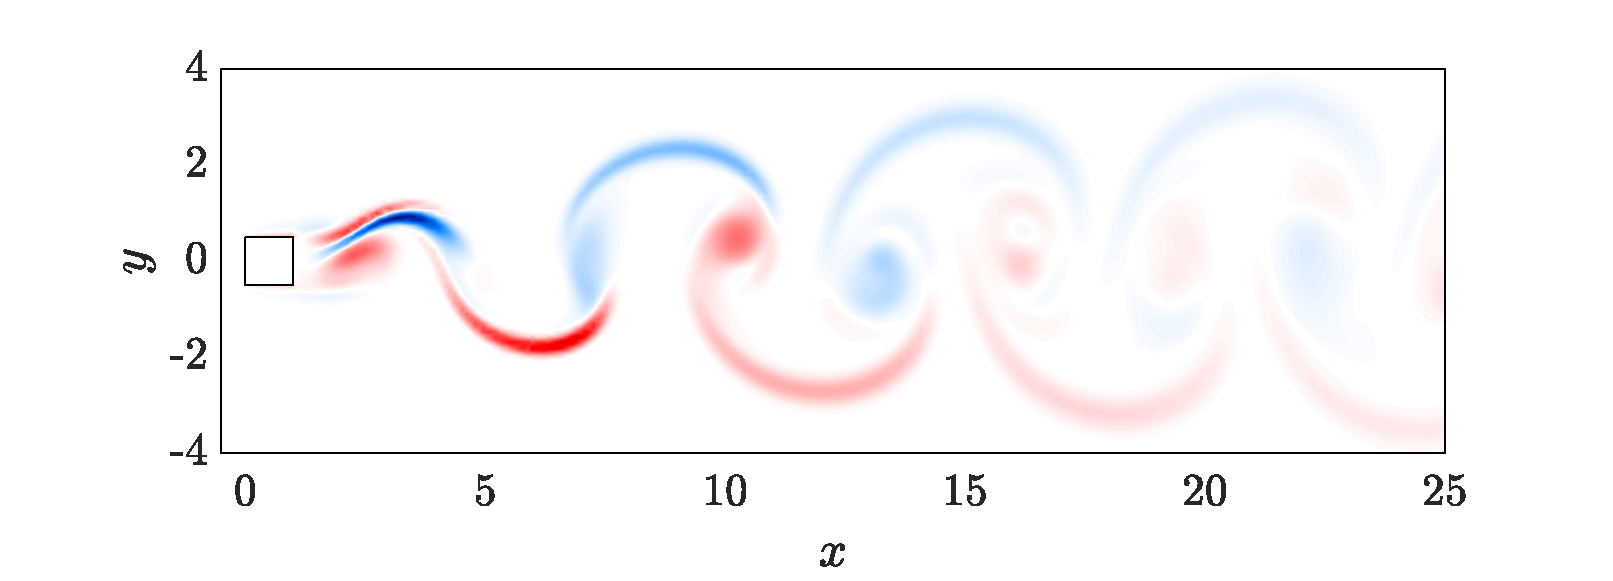
\includegraphics[width=0.49\textwidth]{./fig/AR1/omegax_Re200_beta_1p5_modeA.eps}
  \includegraphics[width=0.49\textwidth]{./fig/AR1p25/omegax_Re200_beta_5p5_modeB.eps}
  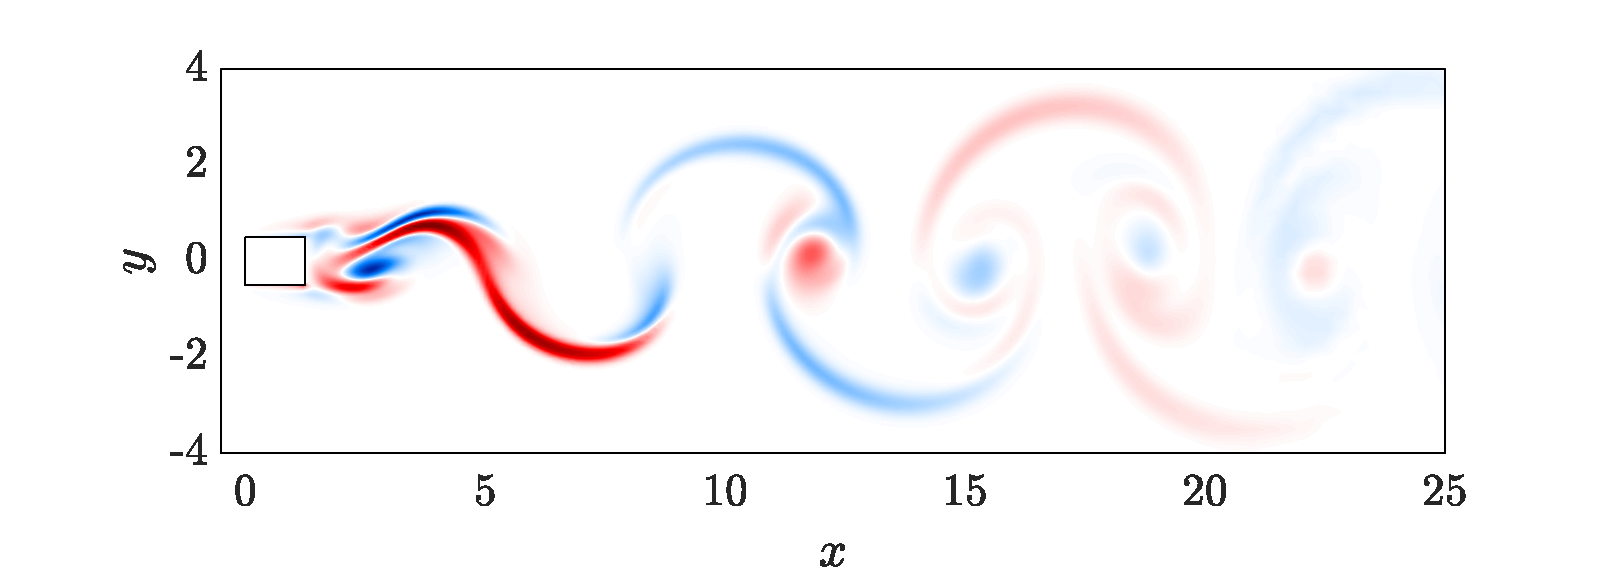
\includegraphics[width=0.49\textwidth]{./fig/AR1p25/omegax_Re230_beta_2p25_modeC.eps}
  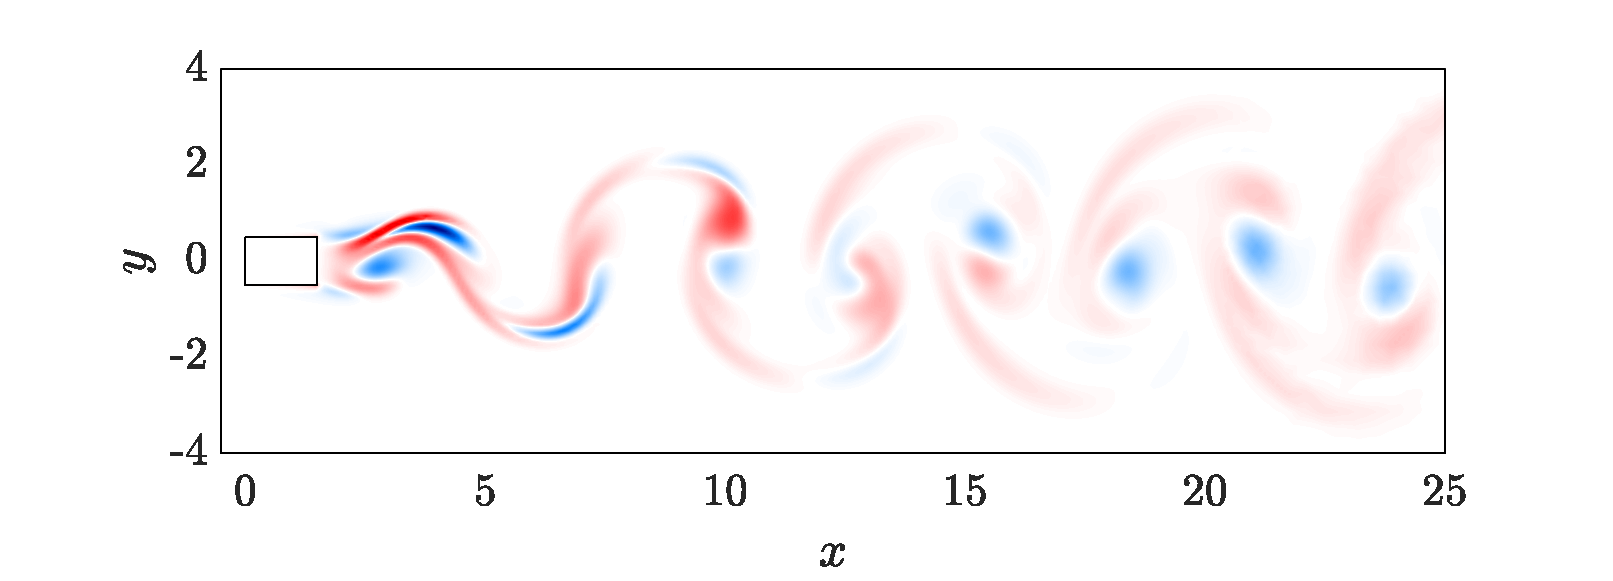
\includegraphics[width=0.49\textwidth]{./fig/AR1p5/omegax_Re200_beta_2p2_modeBp.eps}
  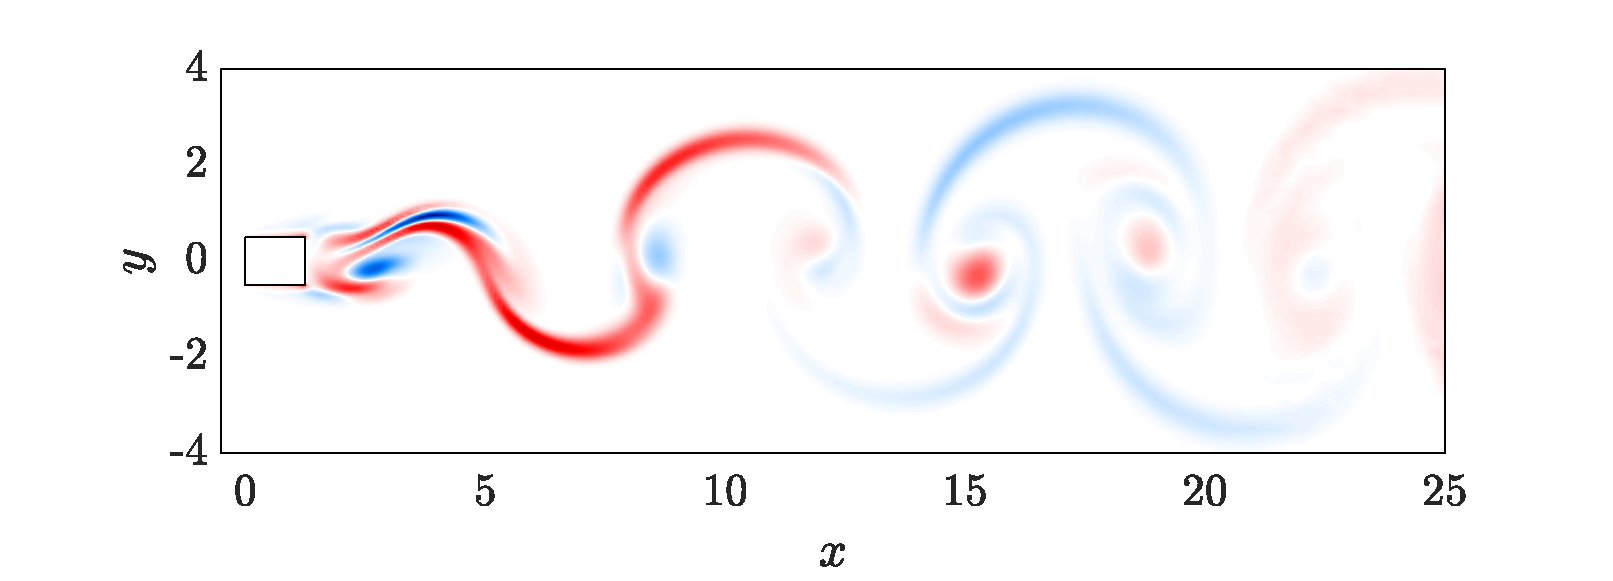
\includegraphics[width=0.49\textwidth]{./fig/AR1p25/omegax_Re230_beta_2p25_modeD.eps}
  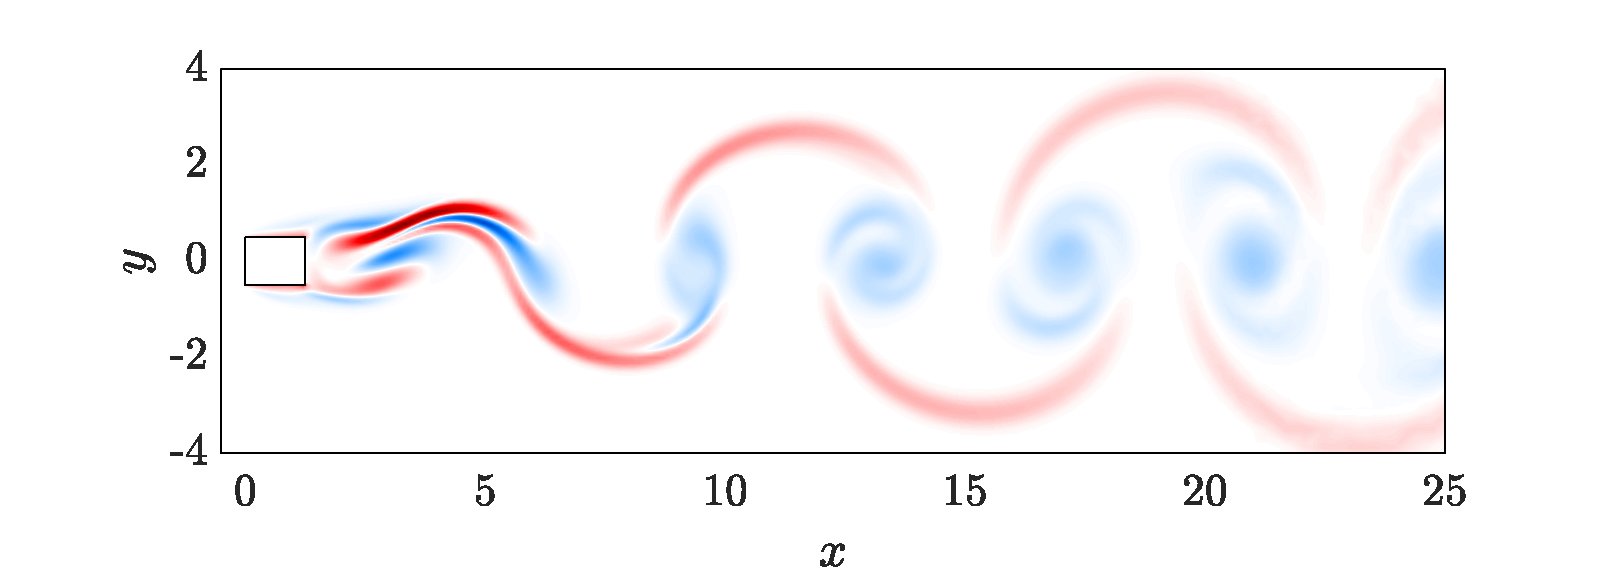
\includegraphics[width=0.49\textwidth]{./fig/AR1p25/omegax_Re240_beta_0p5_modeBpp.eps}
  \caption{Spatial structure of the modes for $1 \le AR \le 1.75$ and $175 \le Re \le 250$. Top left: mode A for $\AR=1$, $Re=200$ and $\beta=1.5$. Top right: mode B for $\AR=1.25$, $Re=200$ and $\beta=5.5$. Centre left: mode QP for $\AR=1.25$, $Re=230$ and $\beta = 2.25$. Centre right: mode $B'$ for $\AR=1.5$, $Re=200$ and $\beta=2.2$. Bottom left: mode QP' for $\AR=1.25$, $Re=230$ and $\beta=2.25$. Bottom right: mode B'' for $\AR=1.25$, $Re=240$ and $\beta=0.5$.}
  \label{fig:modes}
\end{figure}
%
As discussed in \S\ref{sec:intro}, for $\AR=1$, three distinct modes become unstable in rapid succession as the Reynolds number increases. Mode $A$ is the first to become unstable, at $Re \approx 175$, with a characteristic wavelength $\lambda_A \approx 5$ (corresponding to $\beta_A \approx 1.2$). This mode exhibits the following spatio-temporal symmetry:
%
\begin{equation}
\begin{aligned}
\hat{u}(x,y,\beta,t) = &+ \hat{u}(x,-y,\beta,t+T/2) \nonumber \\
\hat{v}(x,y,\beta,t) = &-\hat{v}(x,-y,\beta,t+T/2) \nonumber \\
\hat{w}(x,y,\beta,t) = &+ \hat{w}(x,-y,\beta,t+T/2),
\end{aligned}
\end{equation}
%
which leads to an antisymmetric streamwise vorticity:
%
\begin{equation}
\hat{\omega}_x(x,y,\beta,t) = -\hat{\omega}_x(x,-y,\beta,t+T/2).
\end{equation}

Mode B becomes unstable at $Re \approx 200$, with a much shorter characteristic wavelength $\lambda_B \approx 1$ (corresponding to $\beta_B \approx 5.8$). It satisfies a similar symmetry in the streamwise and cross-stream components, but differs in the spanwise component:
%
\begin{equation}
\begin{aligned}
\hat{u}(x,y,\beta,t) = &+\hat{u}(x,-y,\beta,t+T/2), \nonumber \\
\hat{v}(x,y,\beta,t) = &-\hat{v}(x,-y,\beta,t+T/2), \nonumber \\
\hat{w}(x,y,\beta,t) = &-\hat{w}(x,-y,\beta,t+T/2),
\end{aligned}
\end{equation}
%
resulting in a symmetric streamwise vorticity:
%
\begin{equation}
\hat{\omega}_x(x,y,\beta,t) = +\hat{\omega}_x(x,-y,\beta,t+T/2).
\end{equation}

Finally, Mode QP becomes unstable at the higher Reynolds number $Re \approx 230$, with an intermediate characteristic wavelength of $\lambda_{QP} \approx 2.7$ (corresponding to $\beta_{QP} \approx 2.3$).
%
These results are in excellent agreement with our numerical predictions shown in figures~\ref{fig:mult_AR1_AR1p75}$(a)$ and~\ref{fig:modes}, providing a validation of the computational methodology.

Figure~\ref{fig:mult_AR1_AR1p75}(b-d) illustrates the effect of increasing aspect ratio. As $\AR$ increases, the onset of secondary instabilities is progressively delayed. At fixed $Re$, we observe a consistent reduction in the modulus of the Floquet multipliers associated with the three modes, indicating that the base flow becomes more stable for longer bodies. Quantitatively, the critical Reynolds number increases from $Re_{c2} \approx 175$ for $\AR=1$ to approximately $Re_{c2} = 200-225$ for $\AR=1.75$. This trend is consistent with the delayed onset of the primary instability reported by \citet{chiarini-quadrio-auteri-2021} for increasing $\AR$.

Despite the stabilising effect of elongation, the sequence of bifurcations remains unchanged for $1 \le \AR \le 1.5$, with mode $A$ becoming unstable first, followed by mode $B$. However, mode $QP$ is not detected for $\AR>1.5$ within the range of Reynolds numbers investigated. The characteristic wavelengths of modes $A$ and $B$ exhibit only minor variations with aspect ratio, consistent with the findings of \cite{choi-yang-2014} for $\AR<1$.

In addition to the three established modes, a new mode---denoted $B'$---emerges for $\AR>1$. Mode $B'$ shares the same spatio-temporal symmetry as mode $B$, but has a significantly longer wavelength, comparable to that of mode $A$, see figure~\ref{fig:modes_AR1_AR1p75}. A mode with similar features---both in wavelength and symmetry---was previously reported by \cite{ryan-etal-2006} in the wake of elongated bodies with streamlined leading edges and blunt trailing edges. Within the parameter range considered here, mode $B'$ remains stable for all configurations.

\begin{figure}
  \centering
  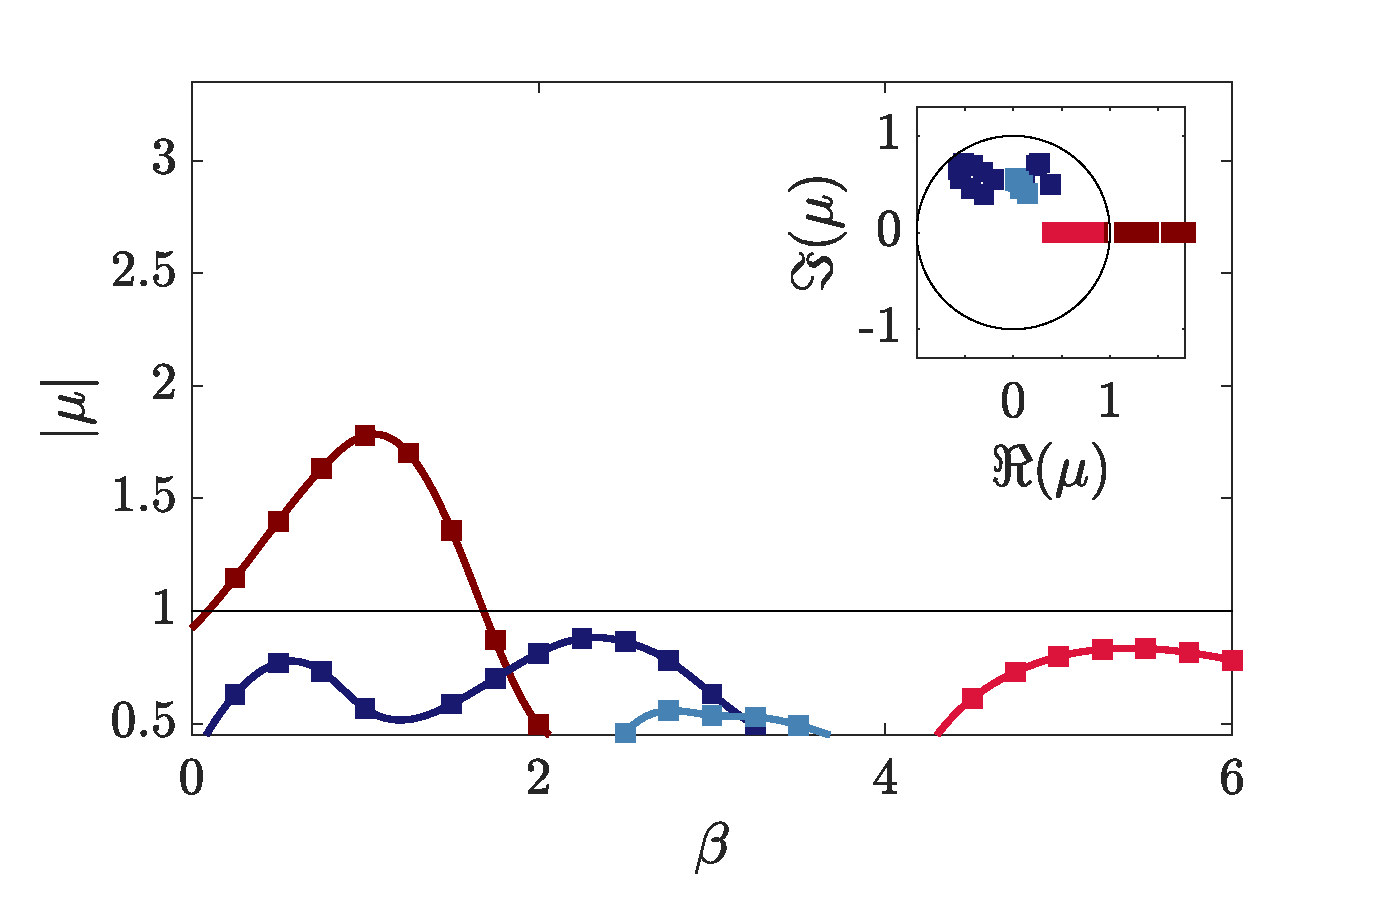
\includegraphics[width=0.49\textwidth]{./fig/AR1p25/mu_beta_Re210.eps}
  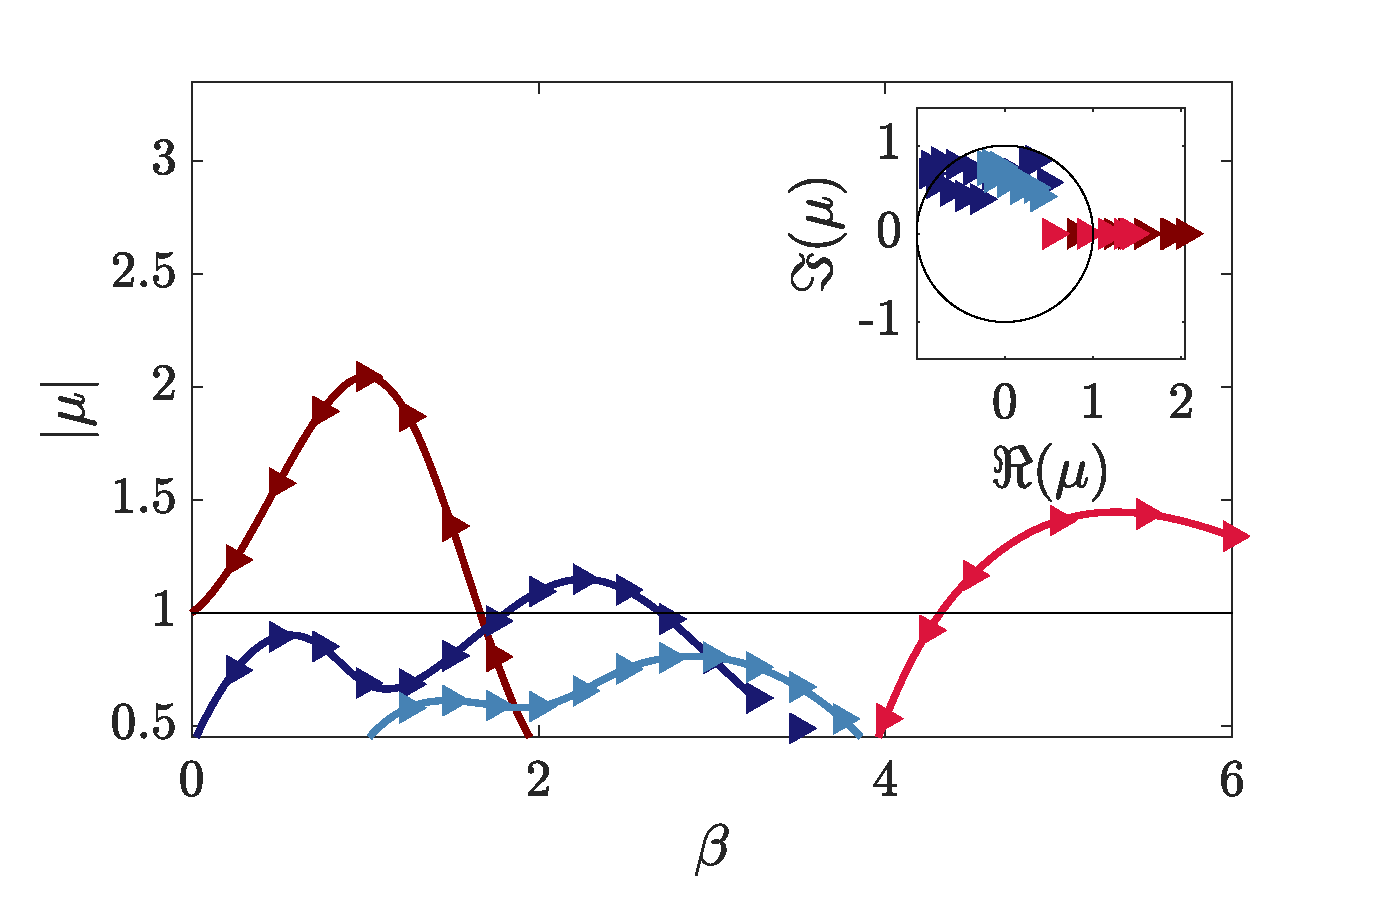
\includegraphics[width=0.49\textwidth]{./fig/AR1p25/mu_beta_Re220.eps}
  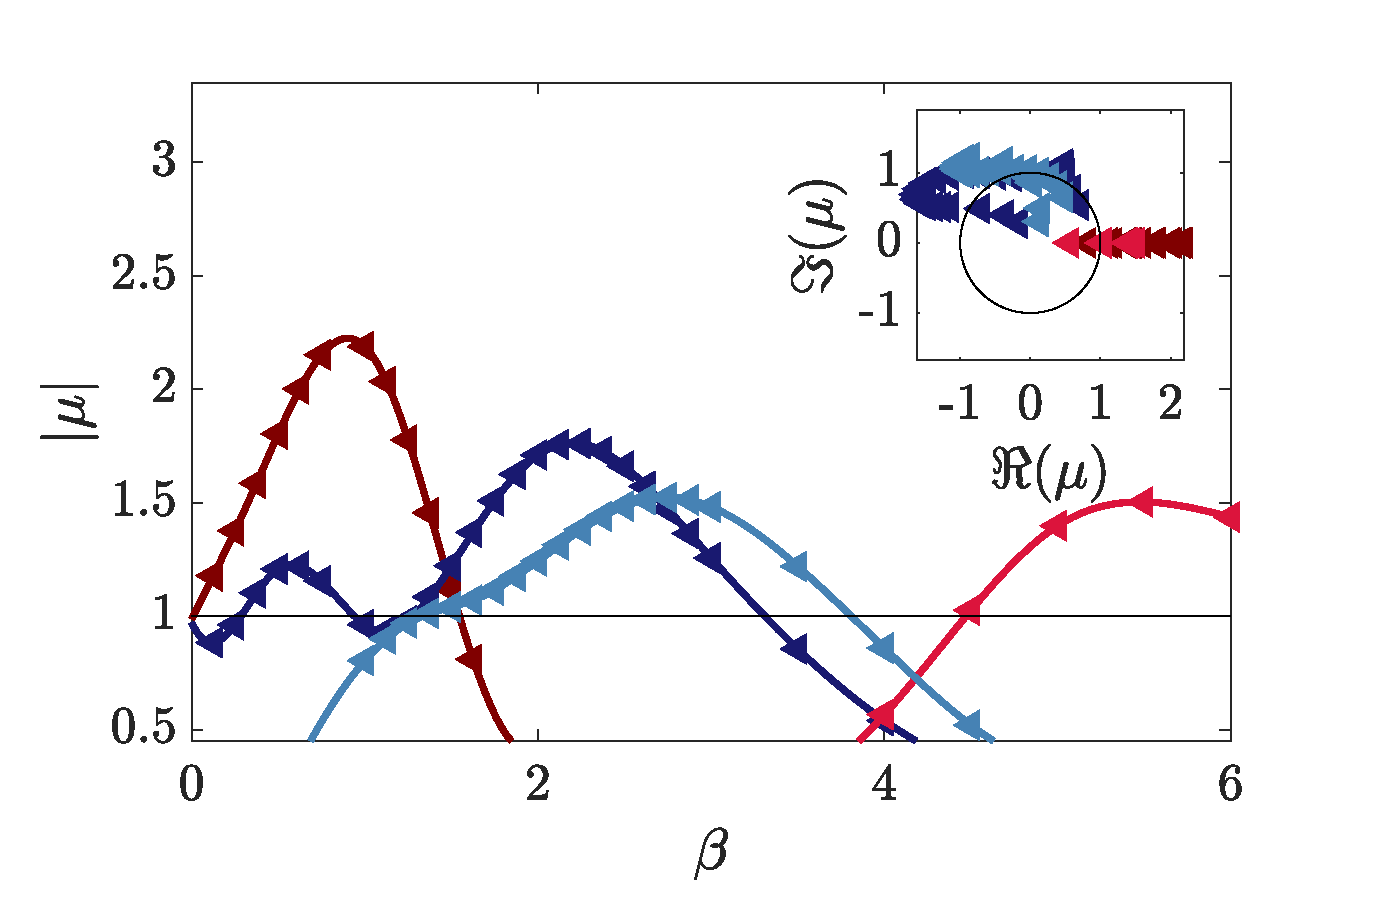
\includegraphics[width=0.49\textwidth]{./fig/AR1p25/mu_beta_Re230.eps}
  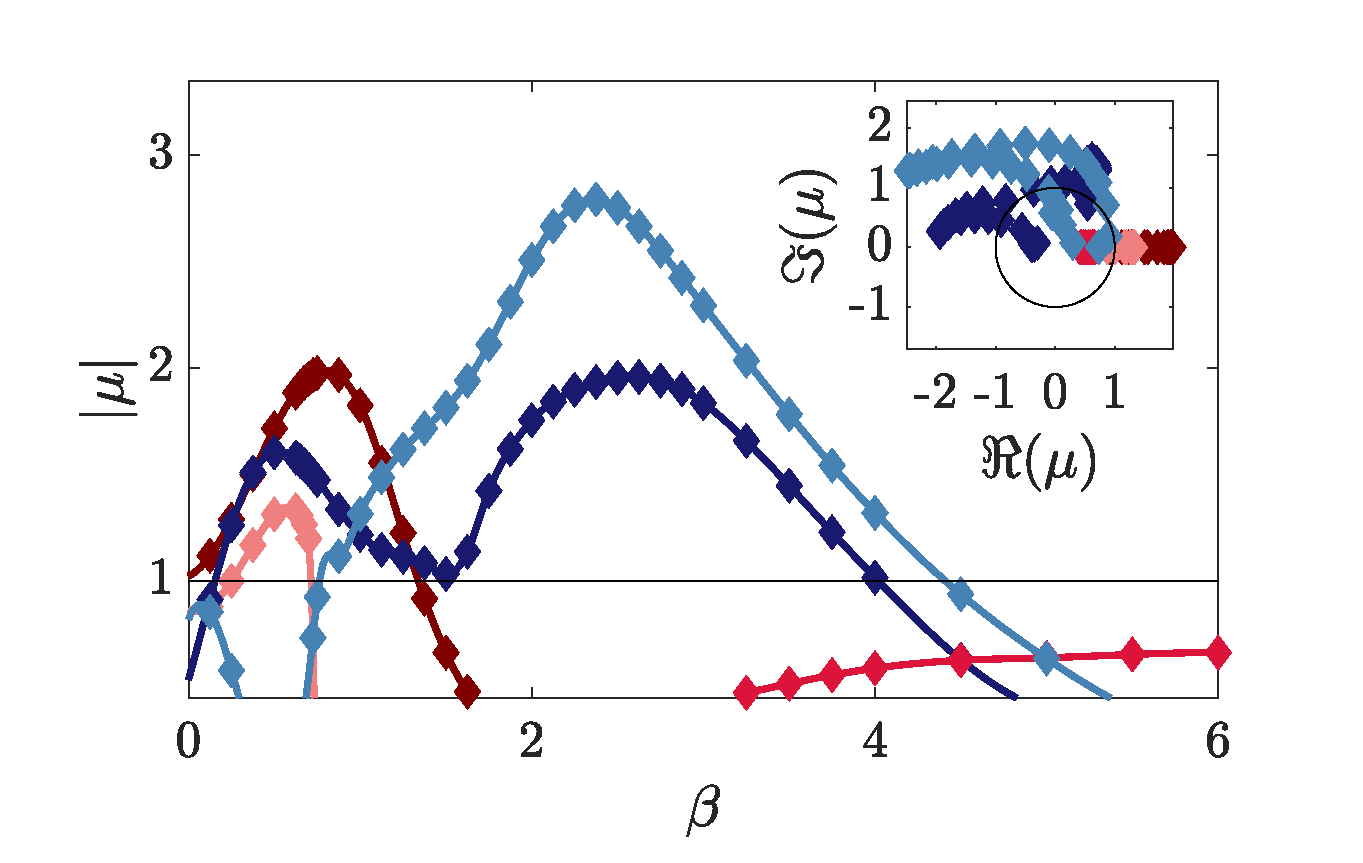
\includegraphics[width=0.49\textwidth]{./fig/AR1p25/mu_beta_Re240.eps}
  %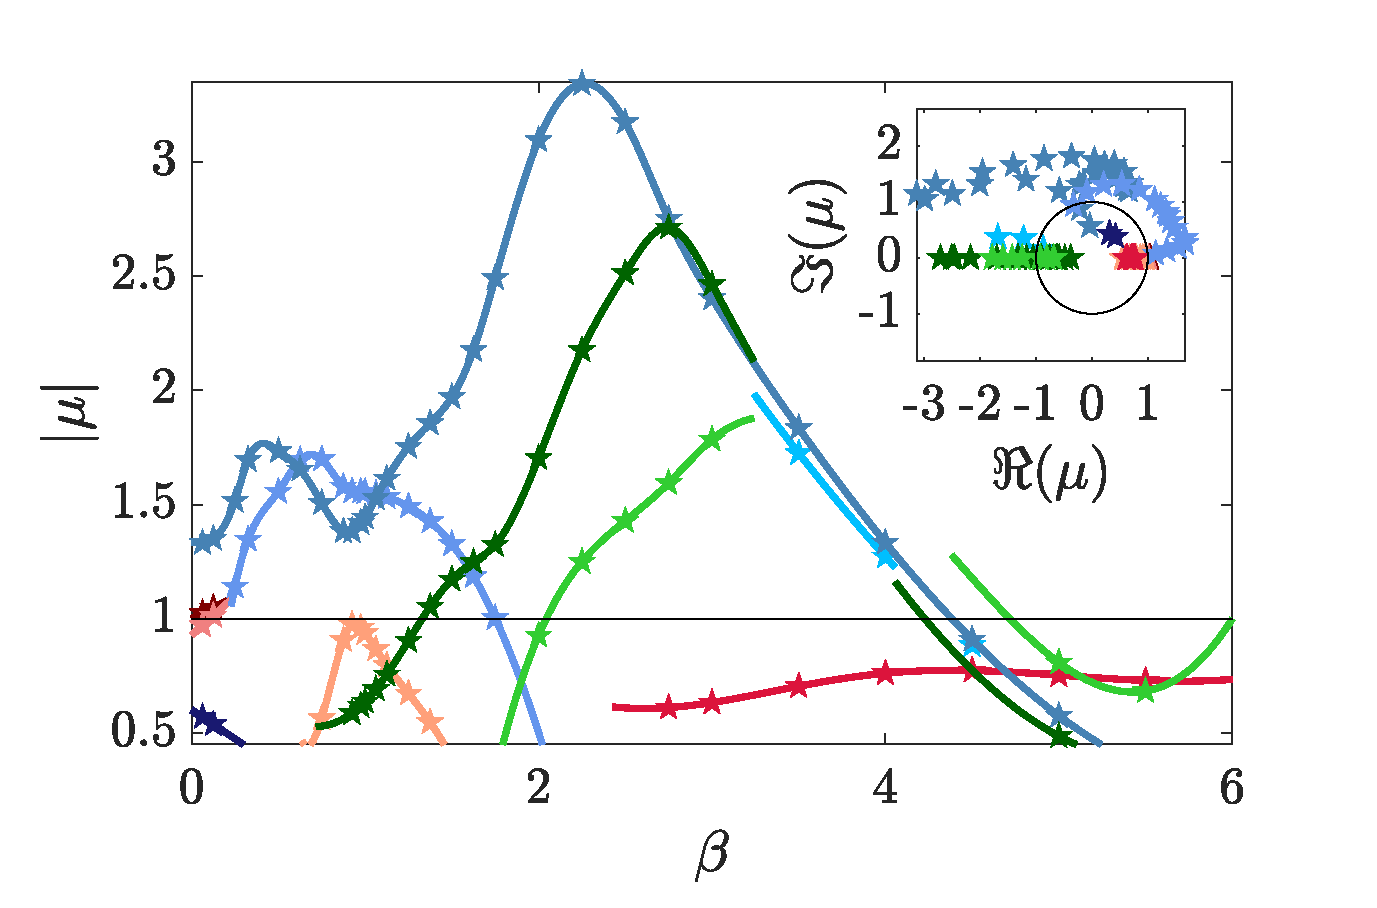
\includegraphics[width=0.49\textwidth]{./fig/AR1p25/mu_beta_Re250.eps}
  \caption{Modulus of the Floquet multipliers for $\AR=1.25$ at different $Re$. In order, the panels are for $Re=210$, $Re=220$, $Re=230$, $Re=240$ and $Re=250$.}
  \label{fig:mult-AR1p25}
\end{figure}
%
Figure \ref{fig:mult-AR1p25} shows the dependence of the Floquet multipliers on Reynolds number for the intermediate aspect ratio $\AR=1.25$, which corresponds to the case where the base flow exhibits the strongest sensitivity to $Re$. The multipliers $\mu_A$ and $\mu_B$ display a non-monotonic dependence on $Re$: both modes $A$ and $B$ are destabilised as $Re$ increases up to approximately $200$, but subsequently restabilise at higher Reynolds numbers. In particular, mode $B$ is stable at $Re \gtrapprox 240$.

For this intermediate $\AR$, additional multipliers cross the unit circle as the Reynolds number increases beyond $Re \gtrapprox 230$. At $Re \approx 230$, a pair of complex-conjugate multipliers with negative real parts and non-zero imaginary parts cross the unit circle, indicating the onset of a new quasi-periodic instability---labelled as mode $QP'$ in figure \ref{fig:modes}(e). Further increasing the Reynolds number to $Re \approx 240$, we observe the emergence of another instability: a real Floquet multiplier with positive real part crosses the unit circle. This mode is synchronous and shares the same symmetry as modes $B$ and $B'$, but has a significantly shorter wavelength, corresponding to $\beta \approx 0.5$, see mode $B''$ in figure \ref{fig:modes}(f). Since these represent higher-order bifurcations of the base flow, their detailed characterisation lies beyond the scope of the present work.

\subsection{Non linear simulations}

XX 3D Simulations for $\AR=1.25, 2, 2.5$ at different $Re$. Show the phase space plots and spectra to characterise the competition between the modes. If needed we can do POD to separate the modes XX

\begin{figure}
  \centering
  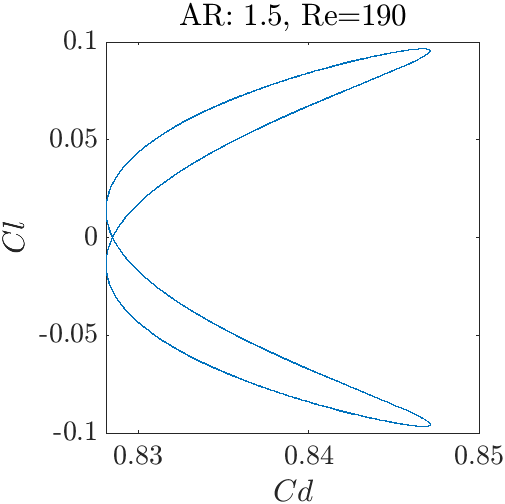
\includegraphics[width=0.24\textwidth]{./fig/nnl/ClCdAR1.5RE190.png}
  \includegraphics[width=0.24\textwidth]{./fig/nnl/ClCdAR1.5RE200.png}  
  \includegraphics[width=0.24\textwidth]{./fig/nnl/ClCdAR1.5RE210.png}
  \includegraphics[width=0.24\textwidth]{./fig/nnl/ClCdAR1.5RE230.png}
  \includegraphics[width=0.24\textwidth]{./fig/nnl/ClCdAR1.5RE250.png}
  %\includegraphics[width=0.49\textwidth]{./fig/AR1p25/mu_beta_Re250.eps}
  \caption{Cl vs Cd for $\AR=1.5$ at different $Re$.}
  \label{fig:ClCd}
\end{figure}

\begin{figure}
  \centering
  \includegraphics[width=0.24\textwidth]{./fig/nnl/psdAR1.5RE190.png}
  \includegraphics[width=0.24\textwidth]{./fig/nnl/psdAR1.5RE200.png}  
  \includegraphics[width=0.24\textwidth]{./fig/nnl/psdAR1.5RE210.png}
  \includegraphics[width=0.24\textwidth]{./fig/nnl/psdAR1.5RE230.png}
  \includegraphics[width=0.24\textwidth]{./fig/nnl/psdAR1.5RE250.png}  
  %\includegraphics[width=0.49\textwidth]{./fig/AR1p25/mu_beta_Re250.eps}
  \caption{Psd for $\AR=1.5$ at different $Re$.}
  \label{fig:ClCd}
\end{figure}

This section describes 3-D wake transition process and mode interactions at different Reynolds number and for different aspect ratios. To this aim, we performed direct numerical simulation XXX DettaigliXXX. The initial condition has a slight effect in determining the exact onset for the instability of modes \cite{jiang-cheng-an-2018}. In this specific case, we started from a 2D solution obtained with a potential solution of the flow, and we initially triggered a disturb of the type XXX. 




Our study started from the smaller aspect ration, $\AR=1.5$. From the Floquet instability analysis of \S \ref{sec:short}, at $Re=200$ the flow becomes unstable due to mode A. For this reason, we performed simulations from $Re=170$ to $Re=250$, with a gap of $\Delta Re=20$.XXX COMPLETE ONCE \S \ref{sec:short} HAS MORE DETAILS AND WE ARE SUREXXX. For each dataset, we computed the streamwise vorticity $\omega_x$ which has been used to characterize the wake. The two dimensional von Kármán wake persist until $Re=210$. From $Re \leq 210$ the wake undergoes a secondary instability leading to a three-dimensional state.

\begin{figure}
  \centering
  \includegraphics[trim={12cm 0 12cm 0},clip,width=0.49\textwidth]{./fig/Wake/AR1.5Re200.png}     
  \includegraphics[trim={12cm 0 12cm 0},clip,width=0.49\textwidth]{./fig/Wake/AR1.5Re210.png}   
  \includegraphics[trim={12cm 0 12cm 0},clip,width=0.49\textwidth]{./fig/Wake/AR1.5Re230.png} 
  \includegraphics[trim={12cm 0 12cm 0},clip,width=0.49\textwidth]{./fig/Wake/AR1.5Re250.png}
  \caption{Isocontours of $\omega_x$ of the three dimensinal wake for $Re=200$ (top-left panel), $Re=210$ (top-right panel), $Re=230$  (bottom-left panel), $Re=250$ (bottom-right panel).}
  \label{fig:wake1.5}
\end{figure}  

 Figure \ref{fig:wake1.5} shows instantaneous $\omega_x=XXX$ isocontours for $Re=210$, $Re=230$, and $Re=250$. At the lowest Reynolds number, the instability is due to mode A.

